\chapter{Literature Review}
% Search for relevant literature
% Evaluate sources
% Identify themes, debates, and gaps
% Outline the structure
% Write your literature review

% Potential Themes:
% Procedural Content Generation
%   Level Generation
%   Randomisation
%   Replayability
%   Search Algorithms
%   Application to AI
%   Image to Image Generation
% Constraint Programming
%   Wave Function Collapse
% Video Games

% Keywords: Video Games, Procedural Content Generation, Wave Function Collapse, Constraint Programming

% What question or problem is the author addressing?
% What are the key concepts and how are they defined?
% What are the key theories, models, and methods?
% Does the research use established frameworks or take an innovative approach?
% What are the results and conclusions of the study?
% How does the publication relate to other literature in the field? Does it confirm, add to, or challenge established knowledge?
% What are the strengths and weaknesses of the research?

% Trends and patterns (in theory, method or results): do certain approaches become more or less popular over time?
% Themes: what questions or concepts recur across the literature?
% Debates, conflicts and contradictions: where do sources disagree?
% Pivotal publications: are there any influential theories or studies that changed the direction of the field?
% Gaps: what is missing from the literature? Are there weaknesses that need to be addressed?

Three key themes identified to be investigated were constraint programming, wave function collapse and procedural content generation. While these themes are presented in three different sections, the ideas discussed heavily overlap.

In summary, Constraint programming and procedural content generation have wide applications and have been a big area of recent research. For example, procedural content generation has seen an increased use of machine learning in recent years, allowing new content to be generated from large dataset models. Similarly, novel constraint programming techniques such as wave function collapse have seen use in generating new output from very limited input data. These techniques are typically applied to video games in order to help create an ever changing experience for the player.

\section{Procedural Content Generation}
\subsection{Overview}
Procedural Content Generation (PCG) describes the use of algorithms to pseudo-randomly generate content. In the context of video games, this randomisation is often used to provide players with variety that can make games more enjoyable to play multiple times. Procedural Content Generation can be used in many facets of video game development. One frequent use of PCG is in randomised level generation. For example, in exploration games such as Minecraft \cite{minecraft} and No Man's Sky \cite{nomanssky}, PCG is used to generate the player's world, offering virtually infinite locations to explore. Other uses include randomising enemy characteristics in Shadow of Mordor \cite{shadowofmordor} and generating randomised weapons in Borderlands \cite{borderlands}. The book `Procedural Content Generation in Games' \cite{pcgbook} is a great resource to read more about PCG.

\begin{figure}[H]
    \centering
    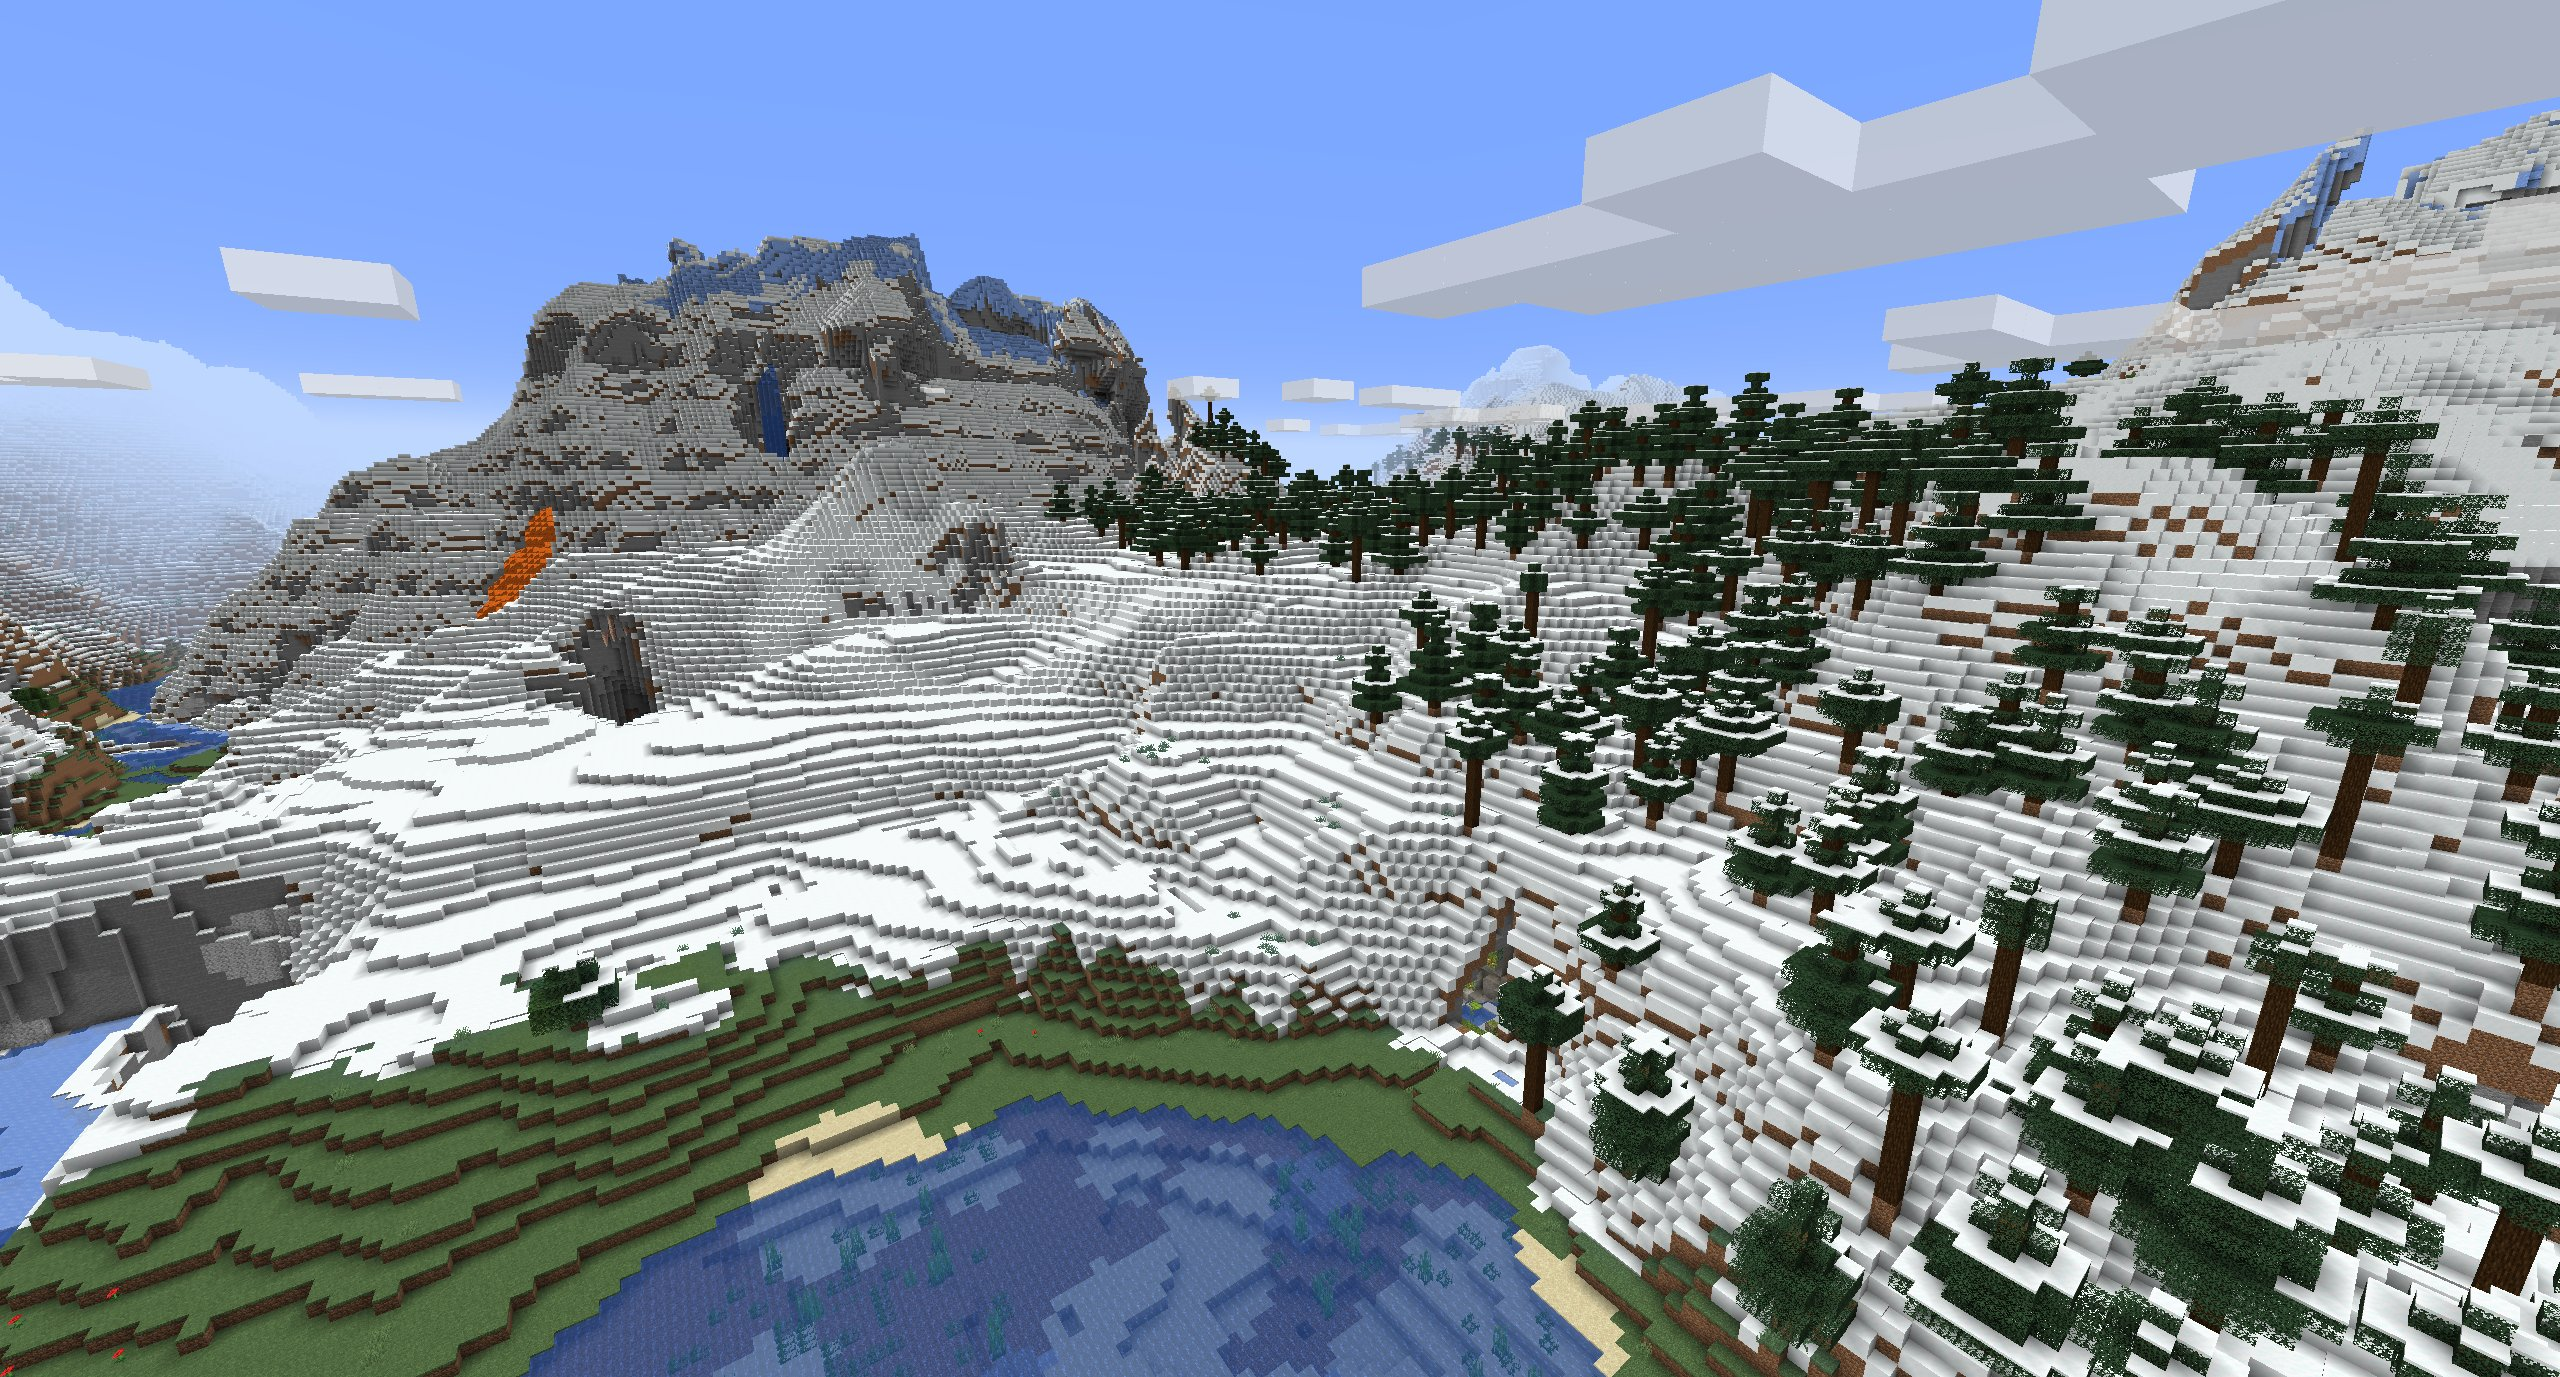
\includegraphics[width=\textwidth, height=0.3\textheight, keepaspectratio]{Images/Minecraft.jpg}
    \caption{Minecraft lets the player explore an infinite, procedural world \cite{minecraft_screenshot}}
    \label{fig:minecraftScreenshot}
\end{figure}

\subsection{Current Applications and Research}
A lot of modern PCG research looks into using AI and machine learning to generate content. Some current applications of machine learning are art, music and code generation as well as chatbots \cite{AIGC_Survey}, text-to-3D synthesis \cite{Magic3D} and even self-driving cars \cite{Self_Driving_Cars}.

\begin{figure}[H]
    \centering
    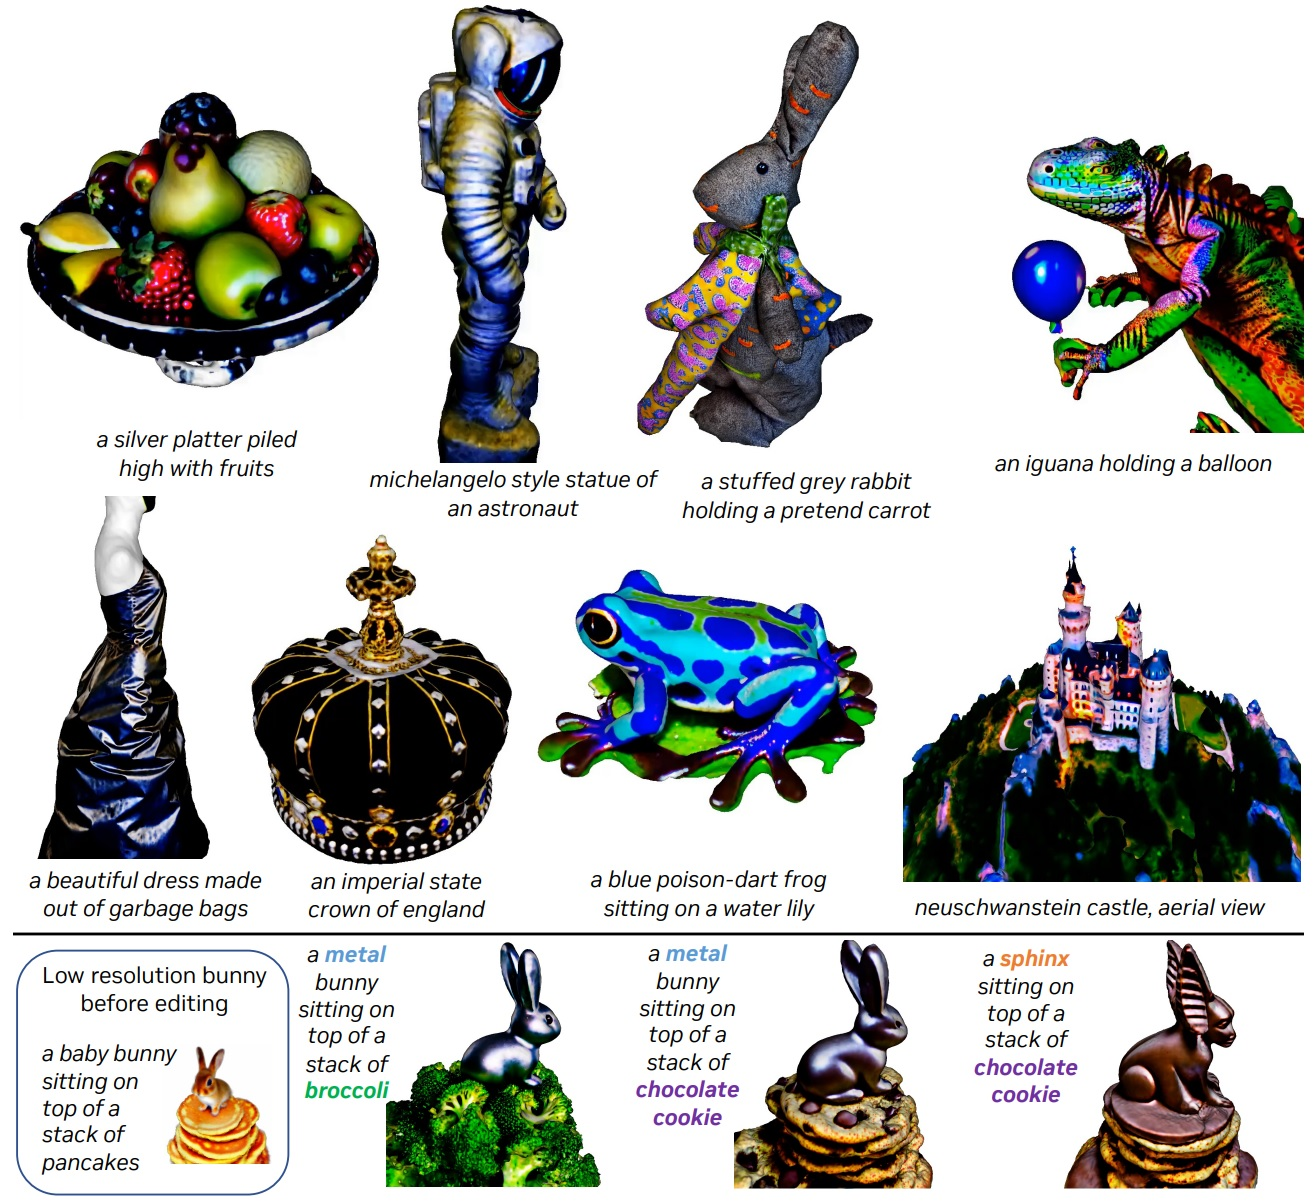
\includegraphics[width=\textwidth, height=0.5\textheight, keepaspectratio]{Images/Magic3D.jpg}
    \caption{Magic3D performs text-to-3D synthesis \cite{Magic3D}}
    \label{fig:magic3D}
\end{figure}

Applications like Stable Diffusion \cite{Stable_Diffusion} can be used to create high quality text-to-image content, while others such as Magic3D \cite{Magic3D} offers text-to-3D synthesis. In terms of text-to-text, ChatGPT \cite{Chat_GPT} serves as a leading language model that can be used to converse about any topic, while GitHub Copilot \cite{GitHub_Copilot} can generate code snippets from user prompts.

\begin{figure}[H]
    \centering
    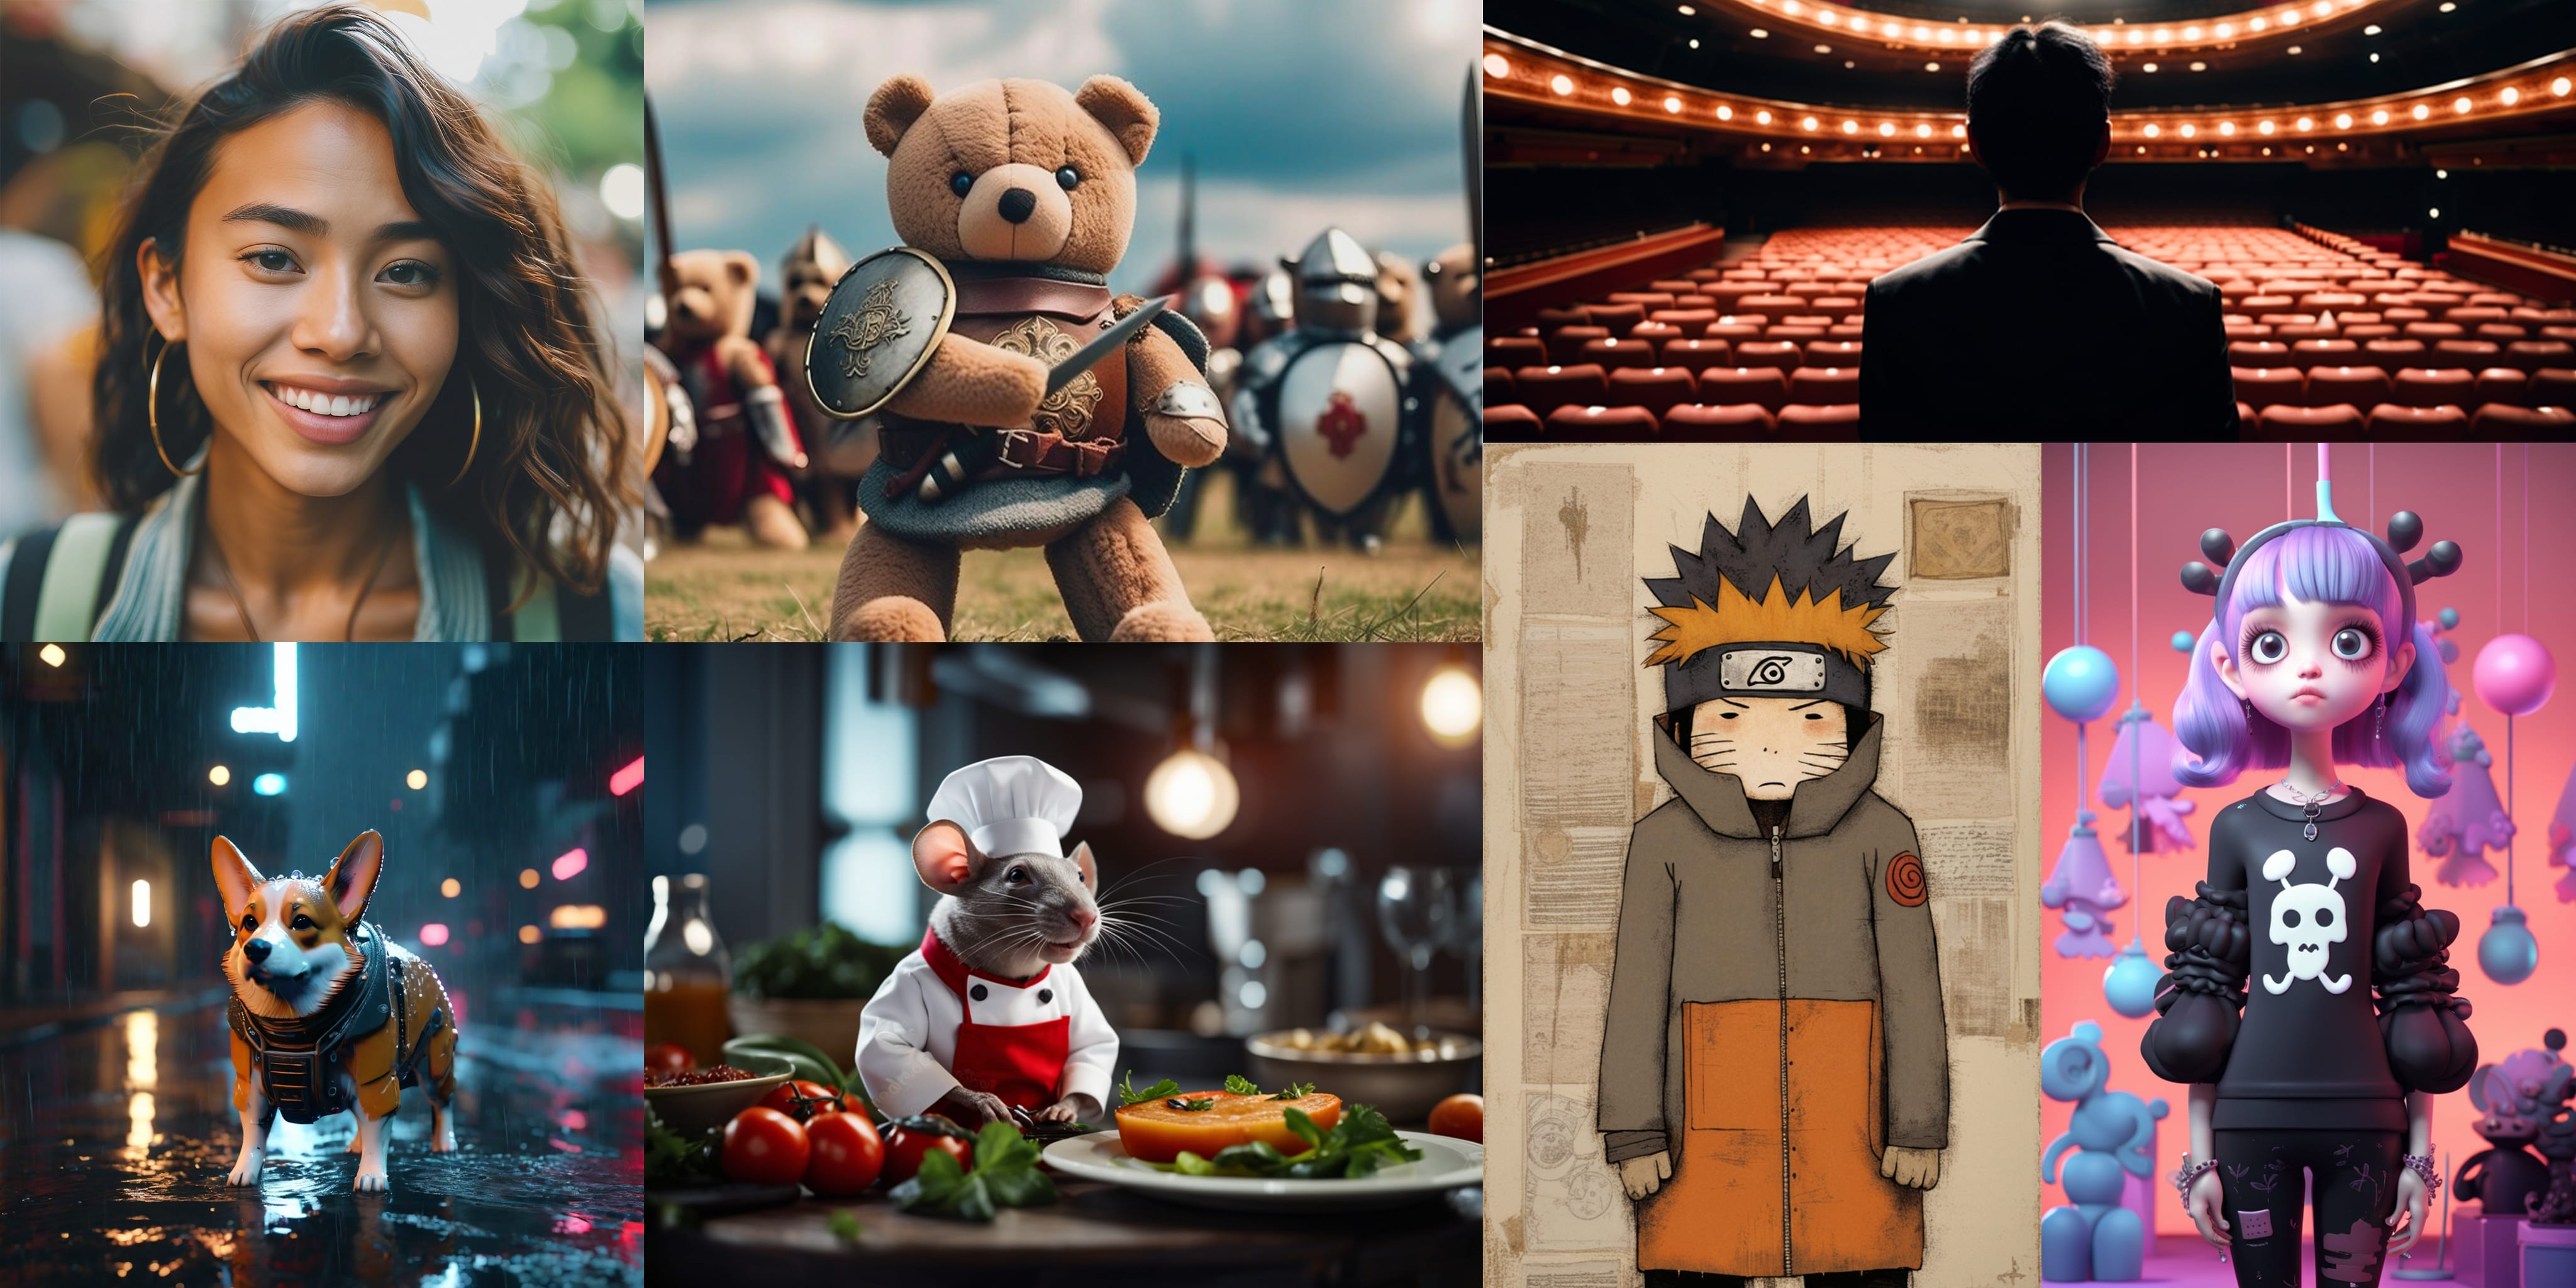
\includegraphics[width=\textwidth, height=0.3\textheight, keepaspectratio]{Images/StableDiffusion.jpg}
    \caption{Stable Diffusion offers text-to-image synthesis \cite{Stable_Diffusion}}
    \label{fig:stableDiffusion}
\end{figure}

In the context of games, machine learning is frequently used in areas like text, character model, texture, music and sound generation \cite{DeepLearningPCG}. Languages such as the Video Game Description Language (VGDL) have even be used to generate entire games using AI \cite{VGDL, VGDL_ASP}. However, by themselves, such languages have limited expressiveness, making it difficult to create interesting games \cite{VGDL}.

\begin{figure}[H]
    \centering
    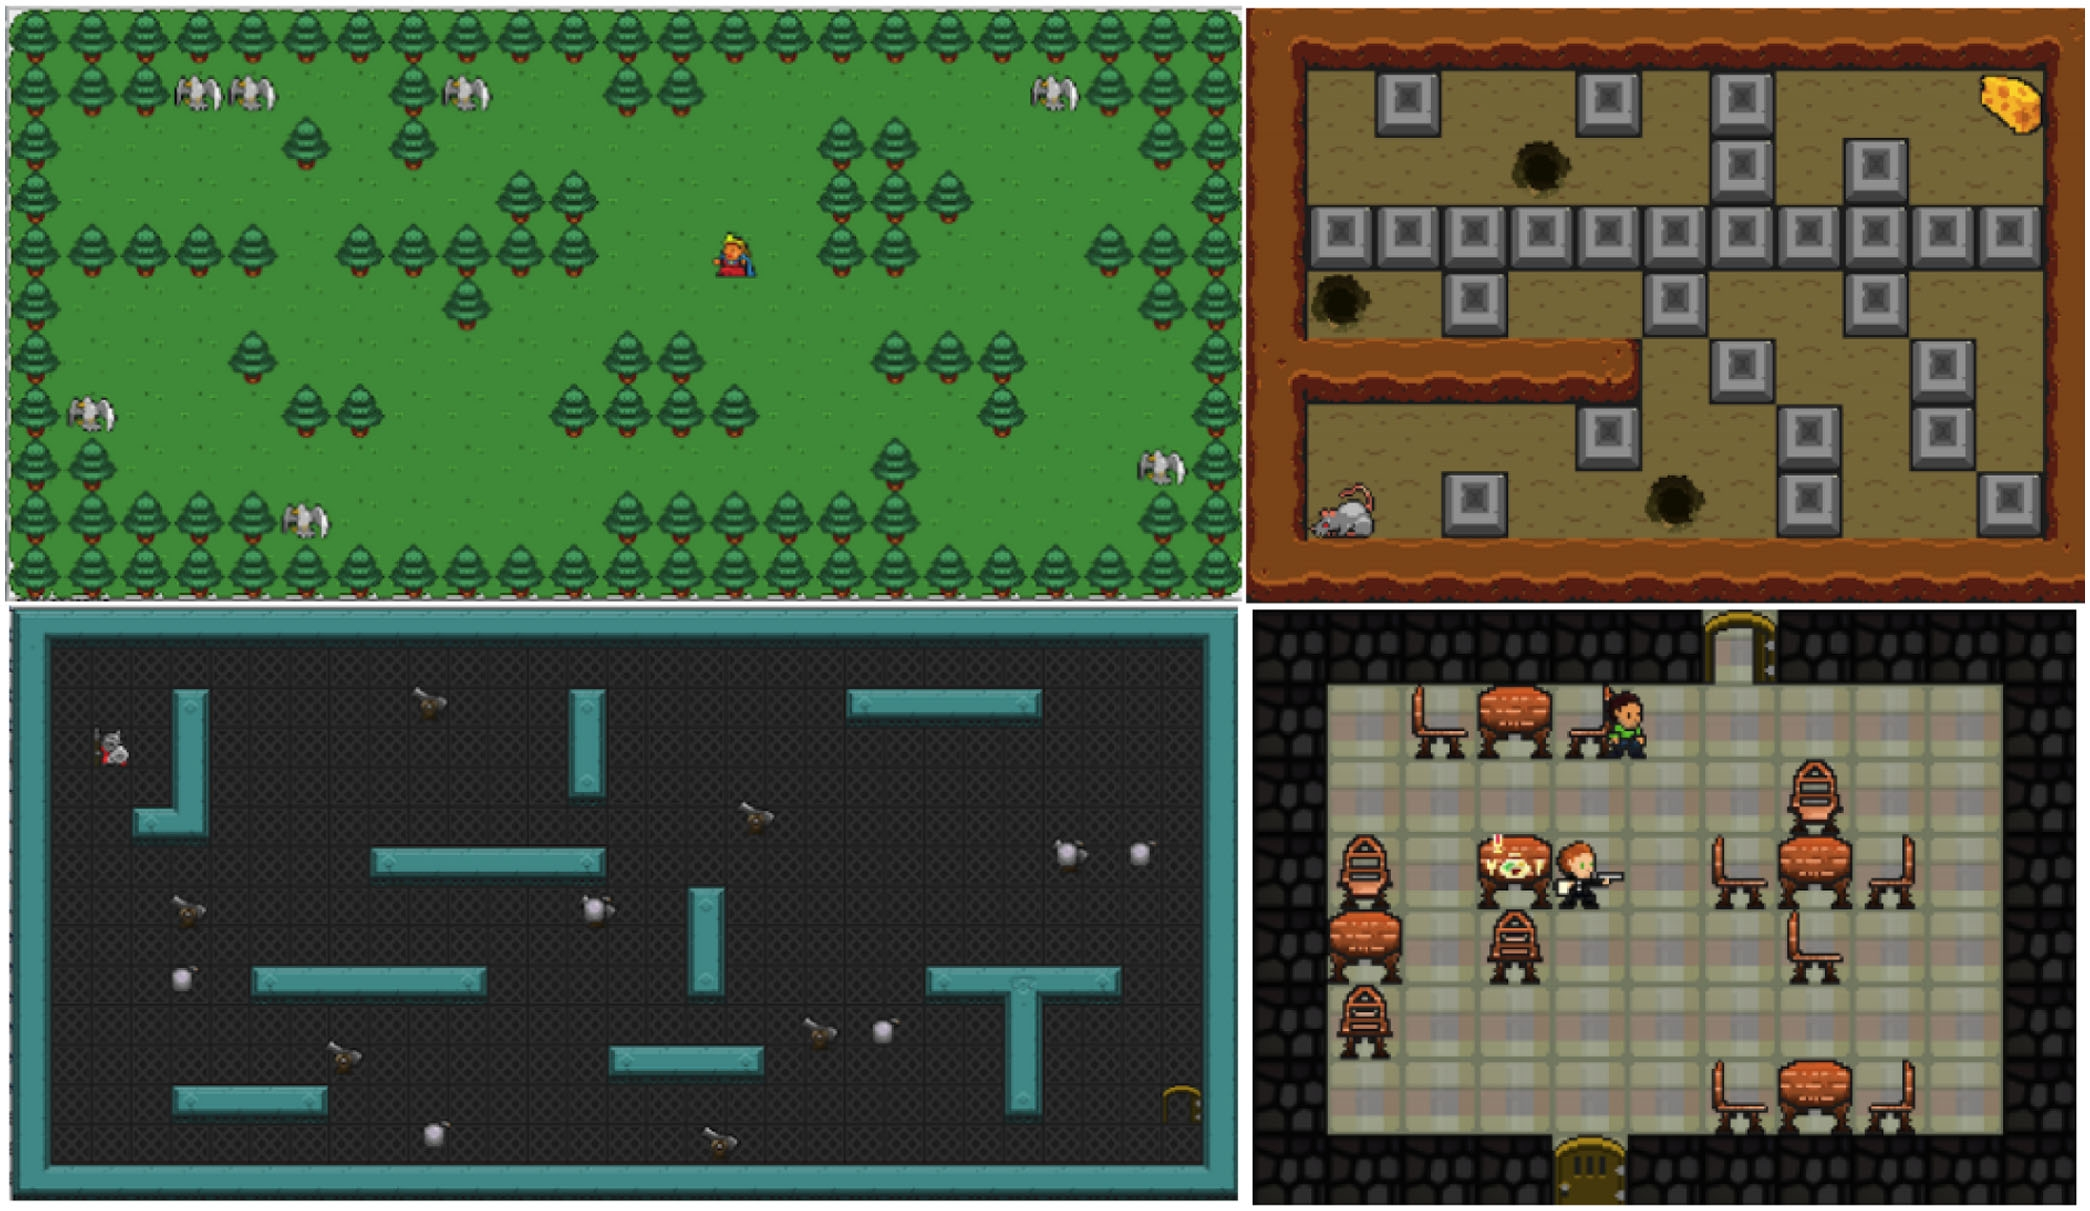
\includegraphics[width=\textwidth, height=0.3\textheight, keepaspectratio]{Images/VGDL.jpg}
    \caption{Games generated using the Video Game Description Language \cite{VGDL}}
    \label{fig:vgdl}
\end{figure}

One paper \cite{CESAGAN} identifies that Generative Adversarial Networks (GANs) can also be used for image generation, but that it is difficult to incorporate constraints. As a solution, it proposes a Conditional Embedding Self-Attention Generative Adversarial Network (CESAGAN). This allows the embedding of a feature vector to the input, enabling the network to model non-local constraints. As a result, this produces higher quality outputs with fewer duplicates. In WFC, it is also difficult to enforce non-local constraints without additional modifications.

\begin{figure}[H]
    \centering
    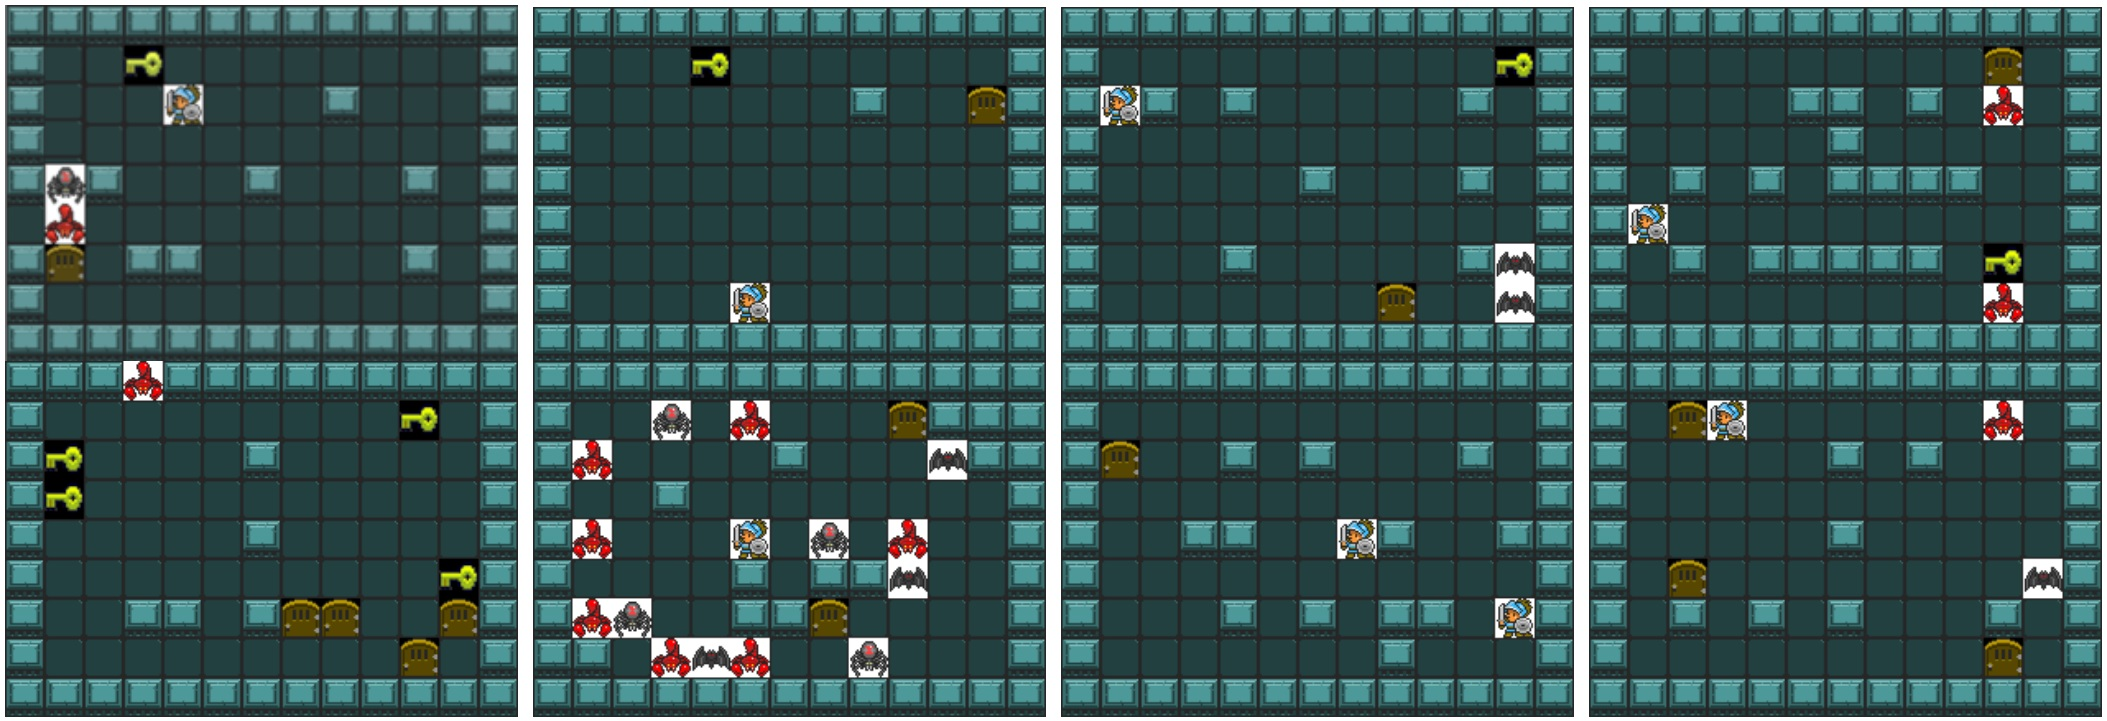
\includegraphics[width=\textwidth, height=0.3\textheight, keepaspectratio]{Images/CESAGAN.jpg}
    \caption{CESAGAN extends upon Generative Adversarial Networks to encourage generation of playable levels requiring additional constraints (top) instead of unplayable levels (bottom) \cite{CESAGAN}}
    \label{fig:cesagan}
\end{figure}

Another transforms 2D level design problems into Markov decision processes \cite{Markov_PCGRL}. This aids reinforced learning to produce high quality output levels. It suggests this reinforced learning could be applied to self-play agents to improve the content generated through simulated playtesting. Three other papers similarly suggest that machine learning is useful for evaluating content through methods like simulated playtesting \cite{DeepLearningPCG, VGDL_ASP, PCGML}. In the context of WFC, it might be useful to apply machine learning content evaluation and adjust the output to increase its quality.

\begin{figure}[H]
    \centering
    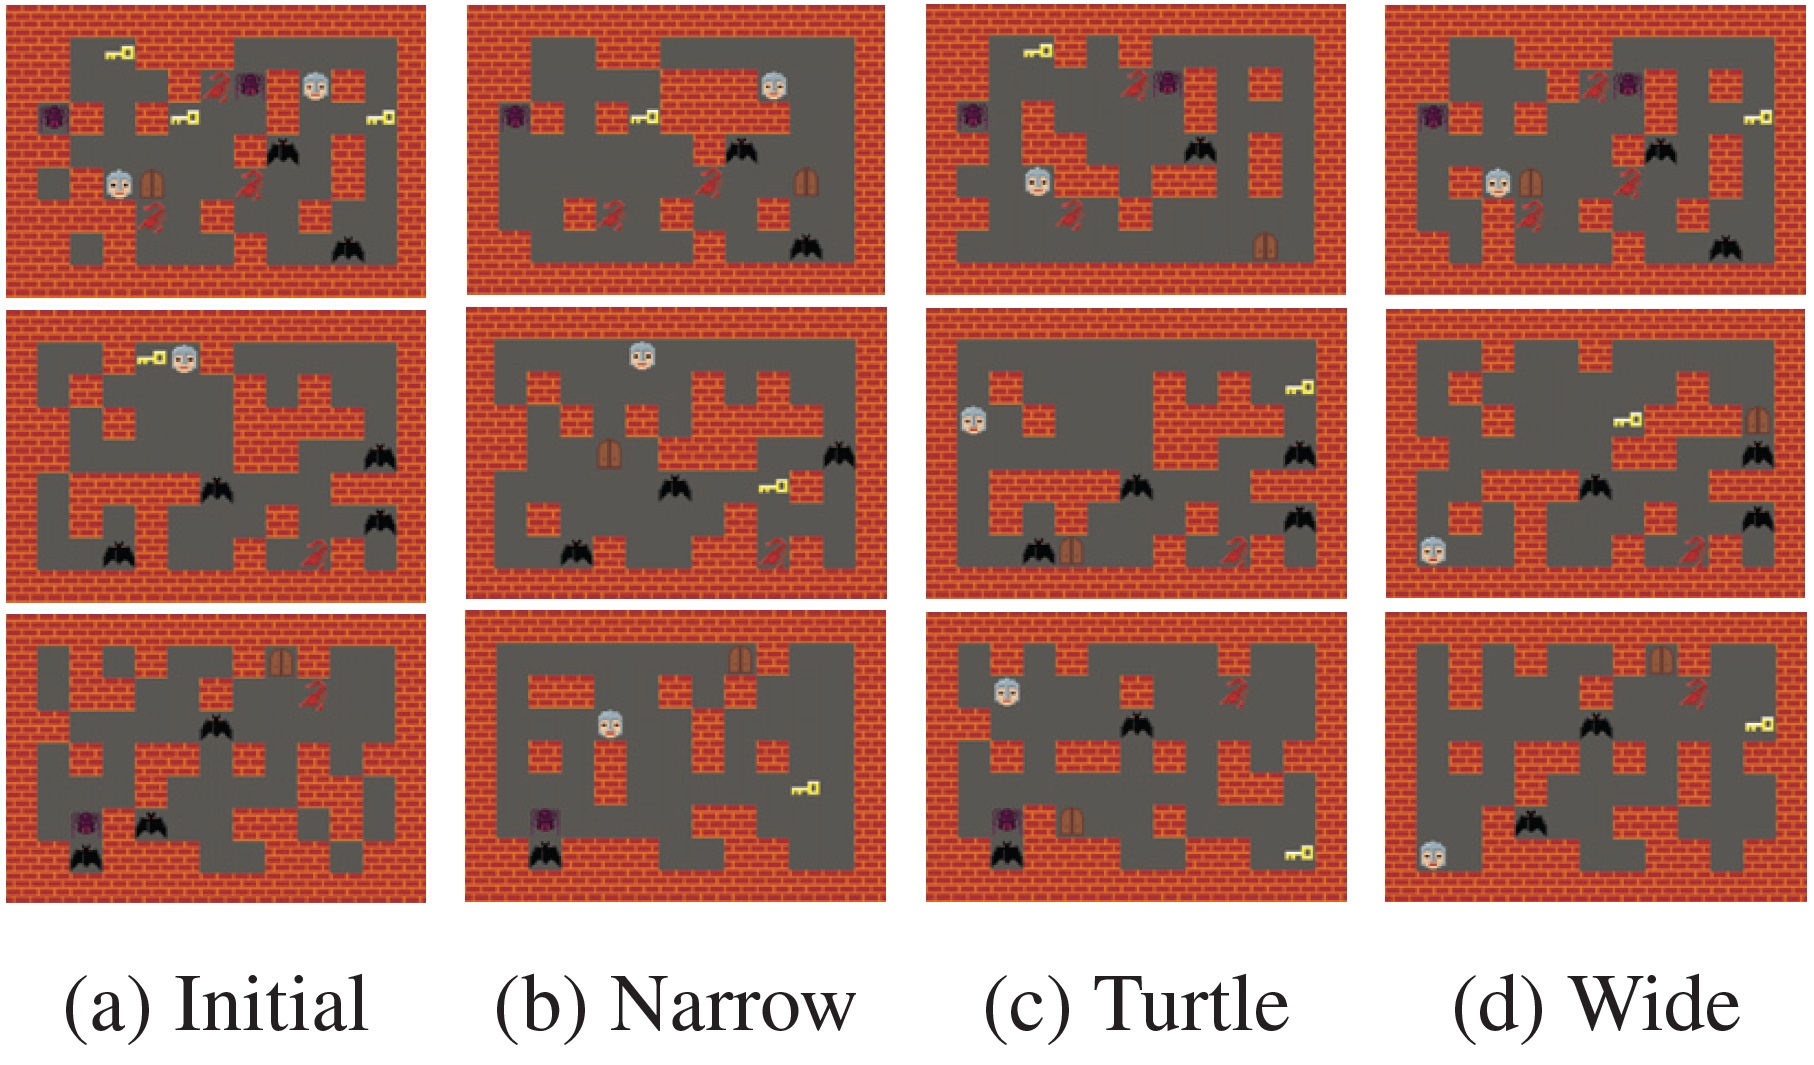
\includegraphics[width=\textwidth, height=0.3\textheight, keepaspectratio]{Images/PCGRL.jpg}
    \caption{Procedural Content Generation via Reinforcement Learning used to create Zelda style levels. An initial random layout (a) is used with three different Markov Decision Process Representations (b), (c) and (d) to create playable levels. \cite{Markov_PCGRL}}
    \label{fig:pcgrl}
\end{figure}

One paper \cite{PCGML} also comments specifically on two limitations of PCG via machine learning. It states that the playability of output produced through machine learning is not guaranteed to be playable, but rather biassed towards generating playable content through the input. The second limitation is that most machine learning has been applied to 2D content. Similarly, whether WFC output is playable or not is not always guaranteed but heavily depends on how the input is defined. Furthermore, the core WFC implementation and many of its offshoots only support 2D content generation \cite{Gumin_Wave_Function_Collapse_2016}. As a result, both machine learning PCG and WFC require carefully tweaked input data and an output evaluator when applied to level generation.

\begin{figure}[H]
    \centering
    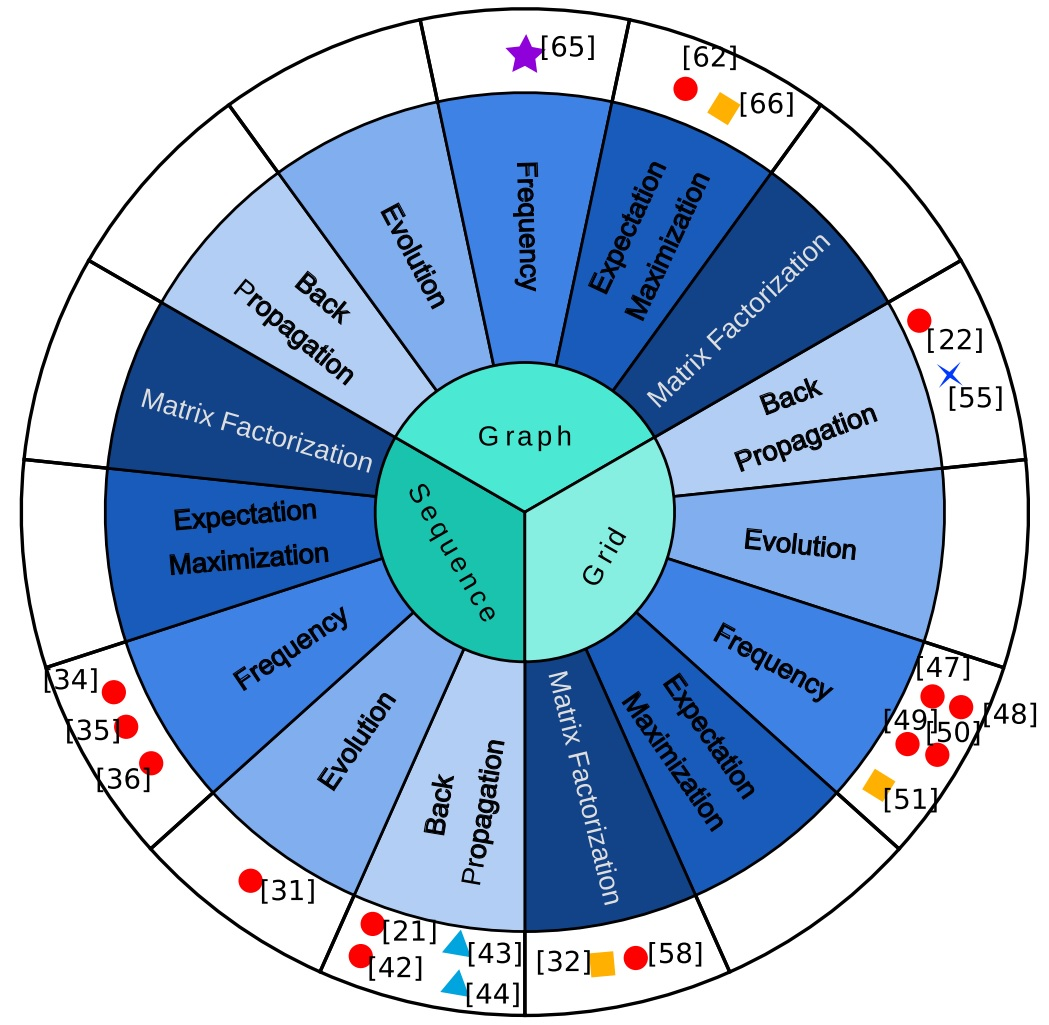
\includegraphics[width=\textwidth, height=0.5\textheight, keepaspectratio]{Images/PCGMLTaxonomy.jpg}
    \caption{A taxonomisation of Procedural Content Generation Machine Learning techniques. There are two categorisations: the underlying data structure (graph, grid, or sequence) and the training method (matrix factorisation, EM, frequency counting, evolution, and backpropagation). Marks are colored for the specific type of content that was generated: red circles are platformer levels, orange squares are ``dungeons,'' the dark blue x is real time strategy levels, light blue triangles are collectible game cards, and the purple star is interactive fiction. Citations for each are listed. Citation numbers correspond to those in the cited paper. \cite{PCGML}}
    \label{fig:pcgml}
\end{figure}



\section{Constraint Programming}
\subsection{Overview}
Constraint programming deals with modelling problems through constraints and then running a solver to find solutions. In the context of PCG and video games, the use of constraints can be useful to tailor the output of PCG as desired and generate new content based on old content. Constraint programming has also been used to solve game tasks. The use of constraints allows for well-defined outputs to be created, but pay for this with more unpredictable generation times when compared to other methods \cite{WFC_In_The_Wild}.

%Discuss some of the problems that constraint programming tackles.
Constraint programming has been applied to a large variety of problem categories, ranging from combinatorial mathematics to logistics and scheduling \cite{CSPLib}.

% Then discuss some current research and identify which problems they attempt to solve.
\subsection{Combinatorial Problems}
For example, three papers take a deeper look into combinatorial problems, which deal with finding an optimal solution among a finite set of possibilities. Deep reinforcement learning has been used to tackle these problems, but it only provides approximate solutions \cite{Combinatorics_CP_RL}. To find optimal solutions, the paper combines deep RL with constraint programming, detailing its use for problems such as the travelling salesman problem with time windows and the 0-1 knapsack problem. Large scale combinatorial problems may have huge search spaces, resulting in low solver performance \cite{Combinatorics_CP_RL}. To address this, it introduces and automated process to add streamliner constraints, which focus effort on searching promising parts of the search space to improve performance. A survey of combinatorial problems and attempts at modelling and solving them effectively identifies, for example, that algorithm selection techniques can achieve significant performance improvements for combinatorial search \cite{Data_Mining_and_Constraint_Programming}. It presents a model for the algorithm selection problem as in Figure \ref{fig:algorithmSelection}.

\begin{figure}[H]
    \centering
    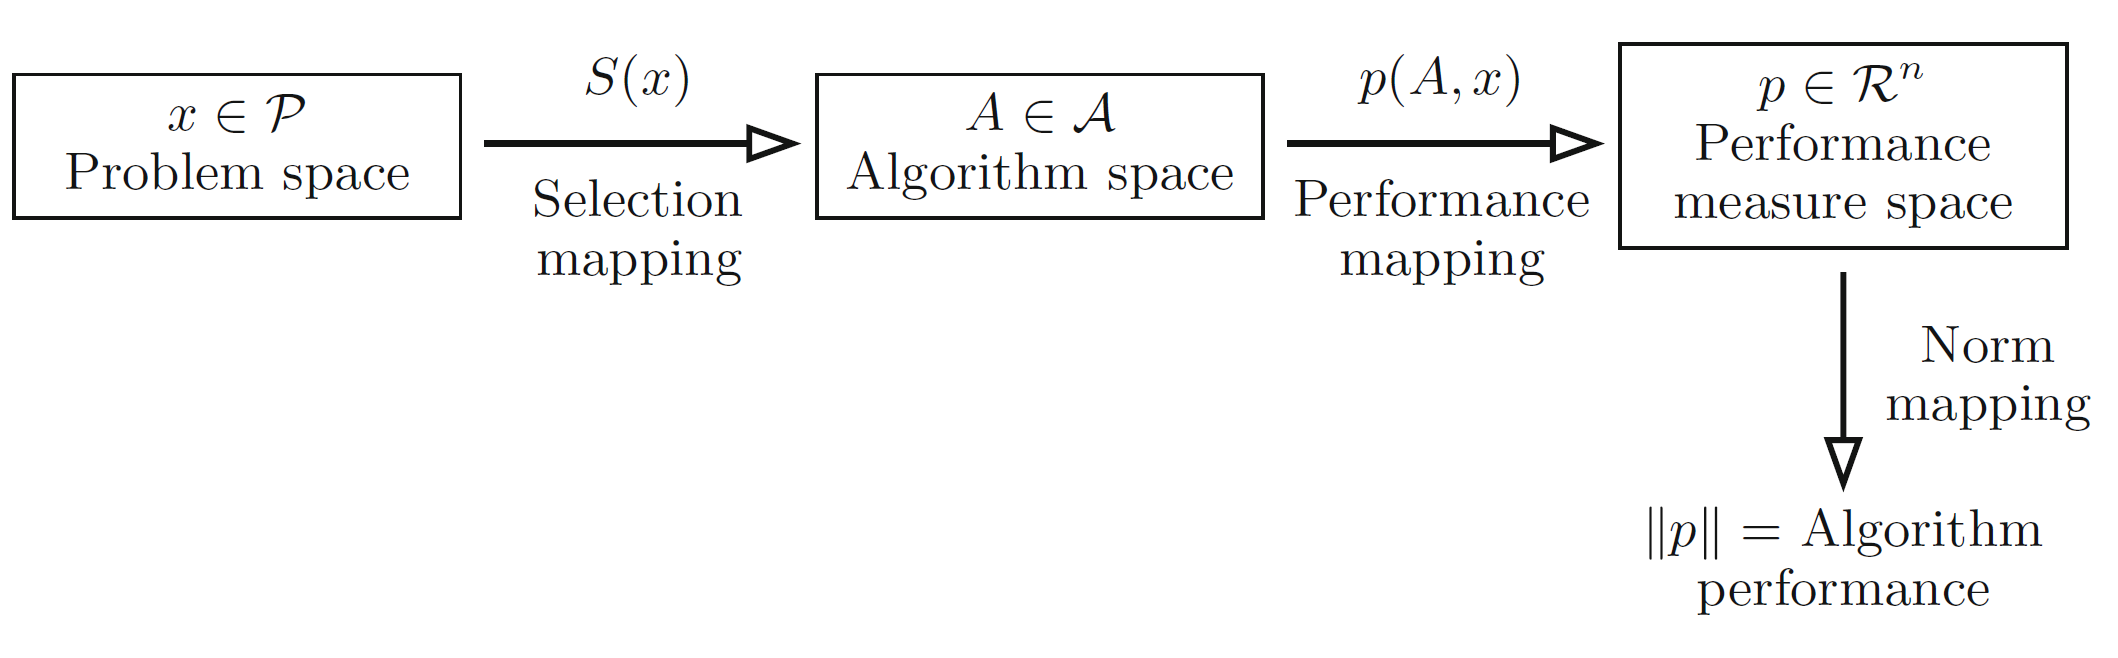
\includegraphics[width=\textwidth, height=0.3\textheight, keepaspectratio]{Images/AlgorithmSelection.png}
    \caption{Basic model for the Algorithm Selection Problem \cite{Data_Mining_and_Constraint_Programming}}
    \label{fig:algorithmSelection}
\end{figure}

Another paper \cite{Metamorphic_Testing} recognises the difficulty in testing constraint solvers due to the vastness of searches they may perform. As a solution, it uses metamorphic testing, which generates new test cases from existing ones. However, it expresses the limitation that this should be used with other forms of testing as metamorphic testing does not recognise when a solver falsely identifies a problem as unsolvable.

\subsection{Logic Programming Languages}
Another interesting application of constraint programming is to AI deep reinforced learning. One paper \cite{Prolog_Deep_Learning} explores the use of the Prolog logic programming language to generate data sets to aid this learning, finding positive results in trained AI agent performance. As part of this process, the paper converts user-specified constraints into Prolog queries through a Python program that generates JSON house plans as in Figure \ref{fig:housePlans}. The pipeline for this is shown in Figure \ref{fig:pythonToProlog}.

\begin{figure}[H]
    \centering
    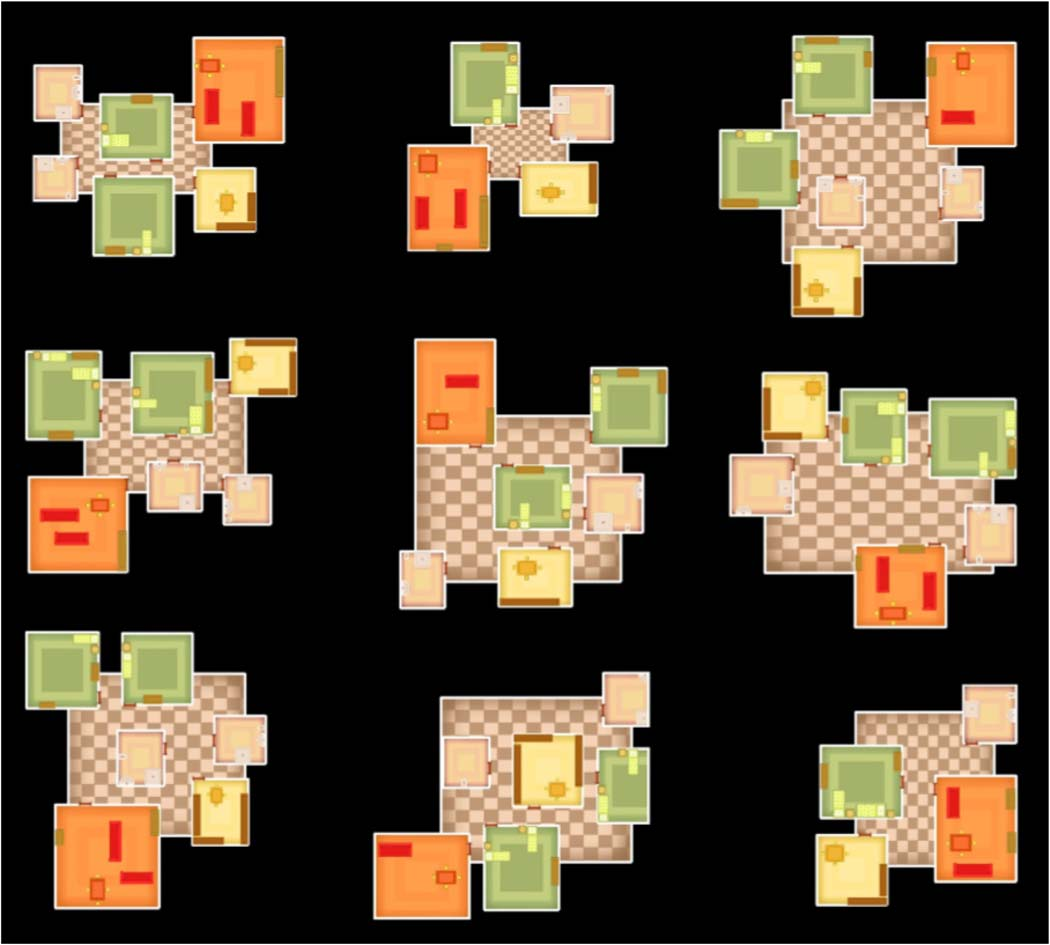
\includegraphics[width=\textwidth, height=0.3\textheight, keepaspectratio]{Images/HousePlans.jpg}
    \caption{Examples of generated house plans \cite{Prolog_Deep_Learning}}
    \label{fig:housePlans}
\end{figure}

\begin{figure}[H]
    \centering
    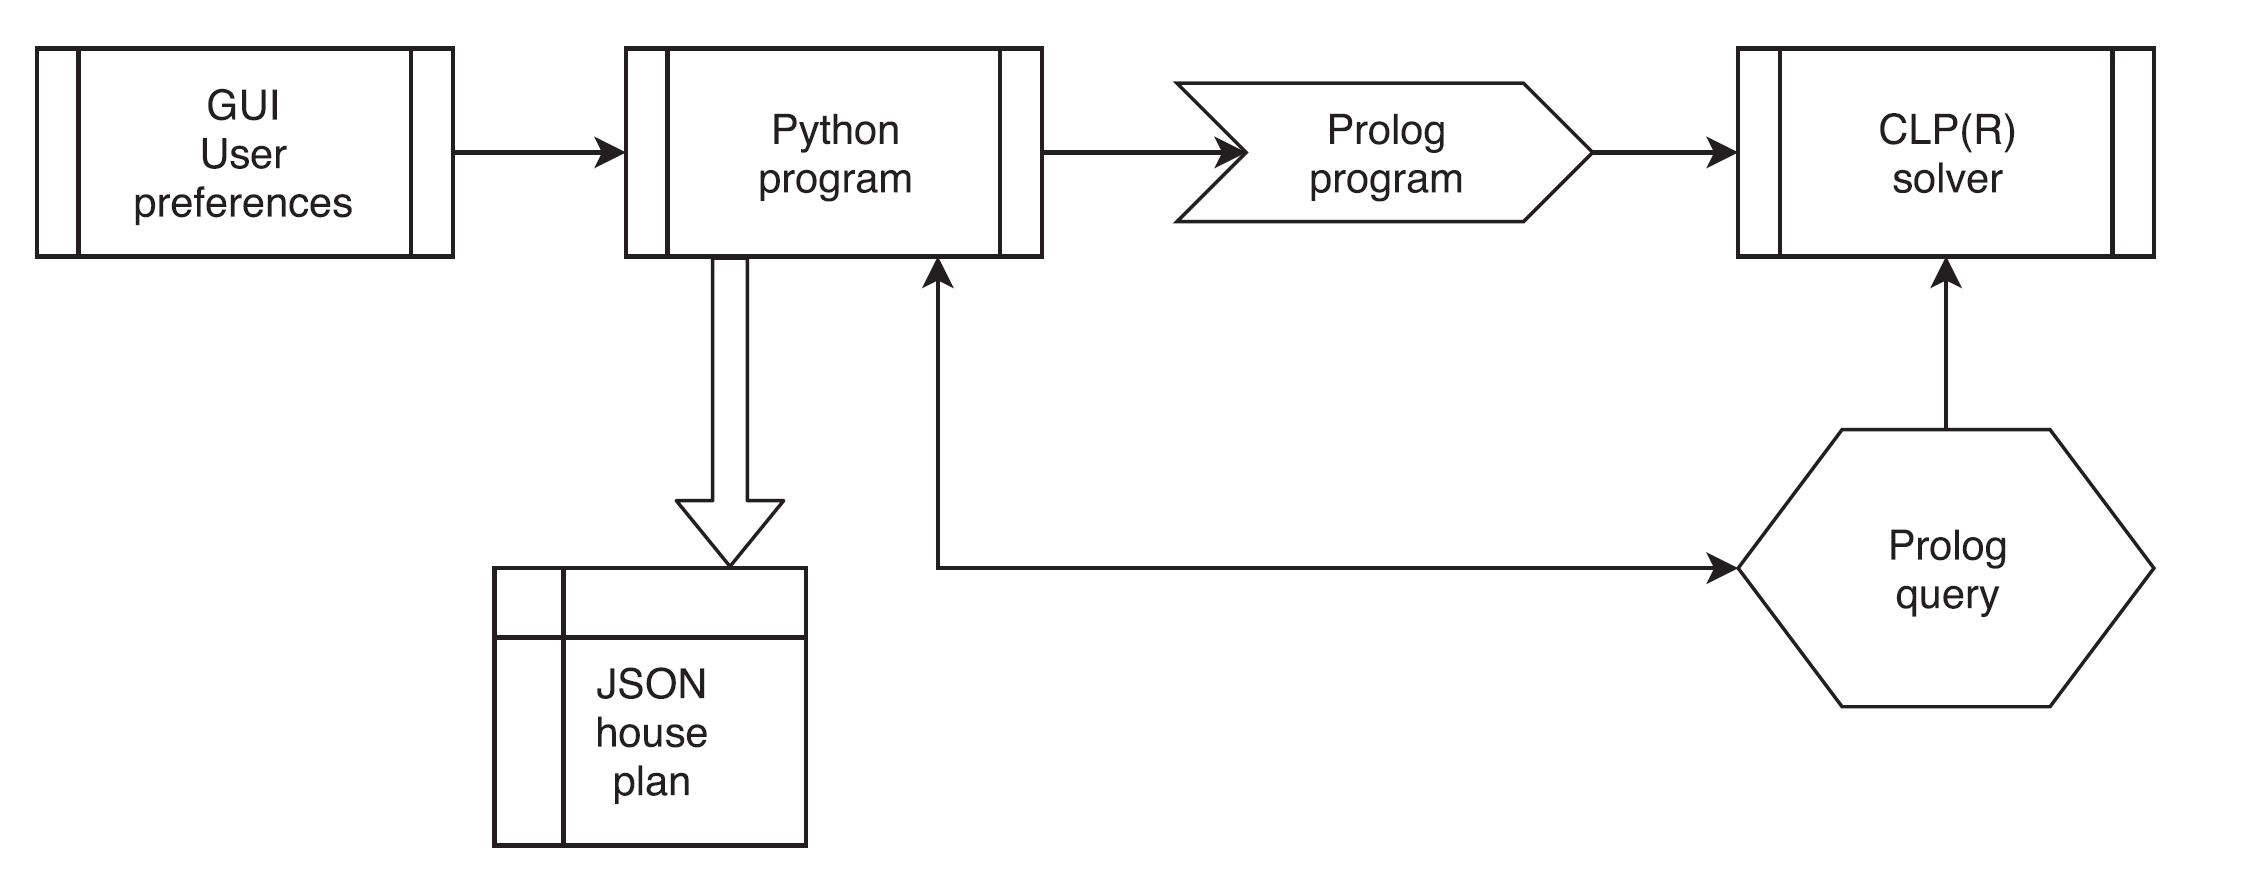
\includegraphics[width=\textwidth, height=0.3\textheight, keepaspectratio]{Images/PythonToProlog.png}
    \caption{Python converting user-specified constraints into Prolog queries \cite{Prolog_Deep_Learning}}
    \label{fig:pythonToProlog}
\end{figure}

Other languages similar to Prolog such as Answer Set Programming (ASP) and the Video Game Description Language (VGDL) extend Prolog's concepts with application to video games. For example, ASP can be used to generate constrained dungeons as in Figure \ref{fig:aspDungeons} \cite{pcgbook}. A range of constraints are encoded. Altars (the golden A tiles) are constrained to have four empty tiles around them. Wall tiles must have at least two neighbouring walls, encouraging the formation of larger wall segments. Gems (the green G tiles) must have three adjacent walls, making them stuck in wall segments. Finally, there must be a path with a minimum length between altars and gems, as well as a path diagonally across the level through this. All of these constraints work together to generate interesting, playable levels.

\begin{figure}[H]
    \centering
    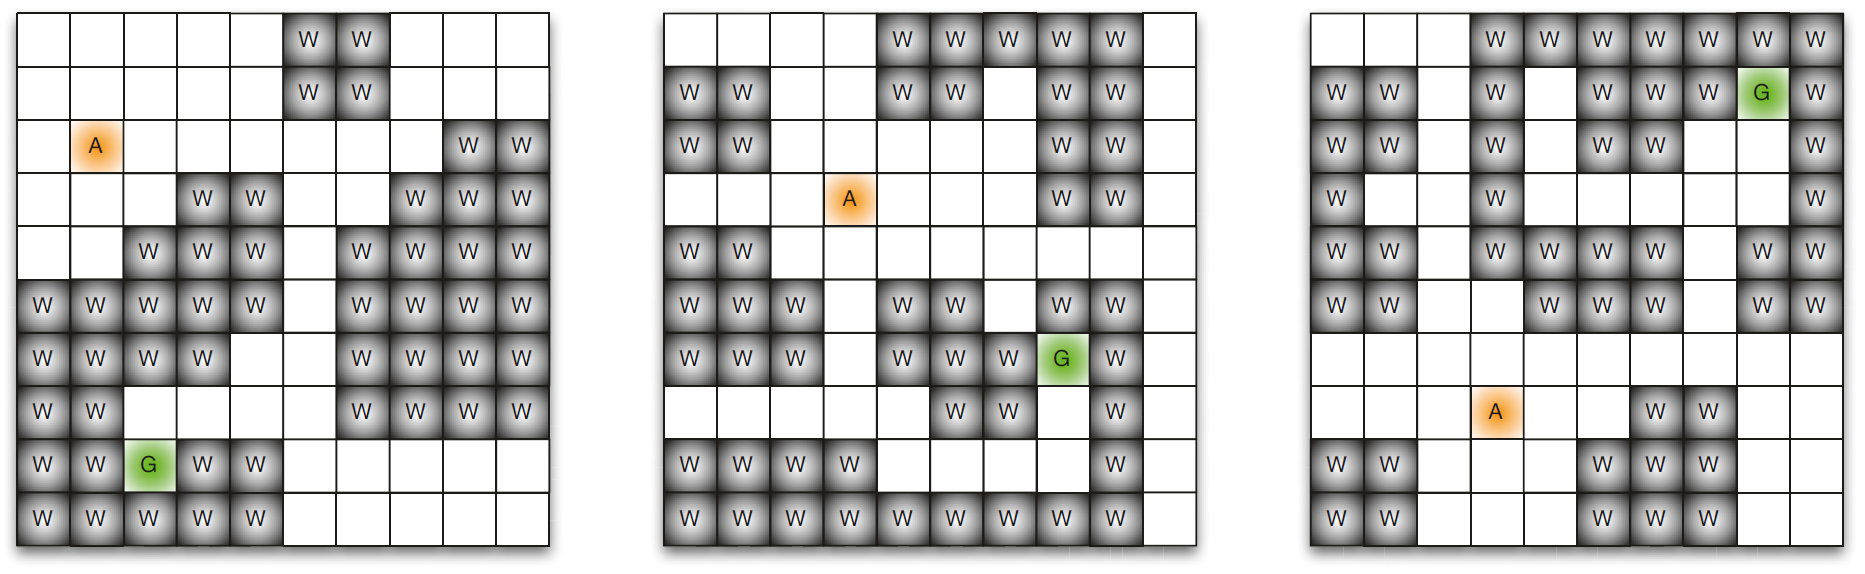
\includegraphics[width=\textwidth, height=0.3\textheight, keepaspectratio]{Images/ASPDungeons.png}
    \caption{Examples of dungeons generated using ASP \cite{pcgbook}}
    \label{fig:aspDungeons}
\end{figure}

One paper \cite{Graph_Constraint_Dungeon} also applies constraint programming to dungeon generation, but instead uses a graph constraint to generate high quality dungeons with distinct areas. Hundreds of variations can be generated from one dungeon with labelled rooms. The dungeon is represented as a graph, which lets areas be selectively turned off and rearranged while meeting design constraints. The concept is shown in Figure \ref{fig:graphDungeon}.

\begin{figure}[H]
    \centering
    \subfigure[The full dungeon]{
        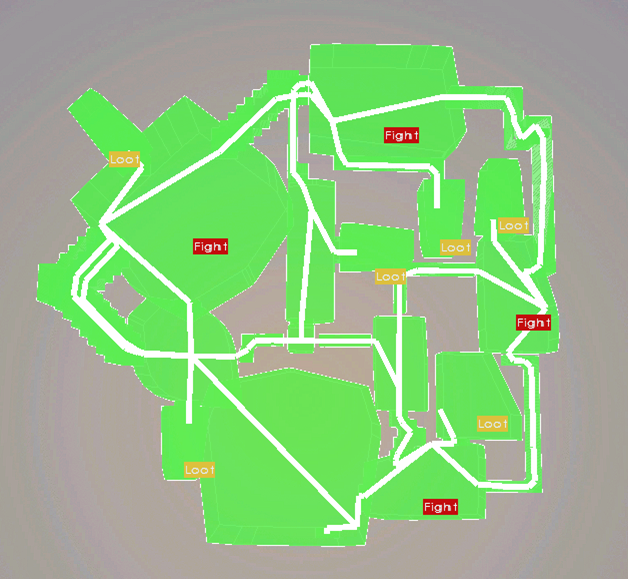
\includegraphics[width=0.475\textwidth, height=0.35\textheight, keepaspectratio]{Images/GraphDungeon1.png}
        \label{fig:graphDungeon1}
    }
    \hfill
    \subfigure[One variation]{
        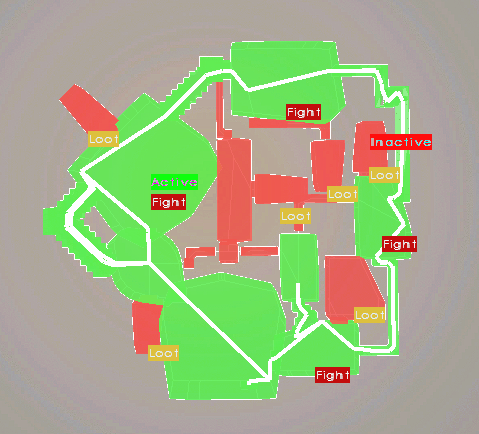
\includegraphics[width=0.475\textwidth, height=0.35\textheight, keepaspectratio]{Images/GraphDungeon2.png}
        \label{fig:graphDungeon2}
    }
    \caption{Generating a variation from a larger dungeon \cite{Graph_Constraint_Dungeon}}
    \label{fig:graphDungeon}
\end{figure}

Another paper \cite{GVG-AI_and_VGDL_Level_Generators} builds on the General Video Game AI framework (GVG-AI) and the Video Game Description Language (VGDL) to create general video game generators. These generators aim to save time by eliminating the need to custom-build a generator for each game. Instead, a game description is given as input and used to generate a level for the game. The results of three generators for a Zelda-style game are shown in Figure \ref{fig:gvgAILevels}. Here, the aim is to collect the key and get to the exit while avoiding attacks by monsters. The player has a sword which can be used to attack monsters and gain additional points.

\begin{figure}[H]
    \centering
    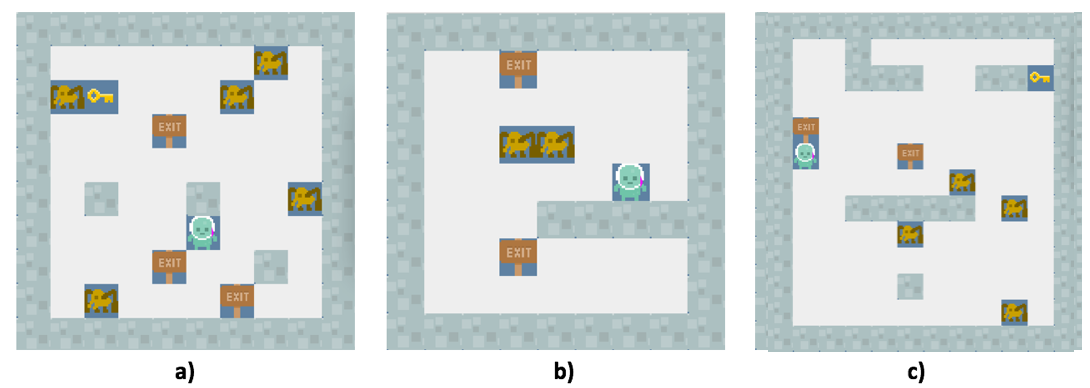
\includegraphics[width=\textwidth, height=0.3\textheight, keepaspectratio]{Images/GVGAILevels.png}
    \caption{Zelda-style levels being generated by a Random Level Generator (a), Constructive Level Generator (b) and Search-Based Level Generator (c) \cite{GVG-AI_and_VGDL_Level_Generators}}
    \label{fig:gvgAILevels}
\end{figure}

\subsection{Further Application to Video Games}
In the context of video games, constraint programming research has looked into applying constraints to PCG and solving game tasks. One recent paper \cite{Plotting_Planning_Problem} aims to solve a planning problem presented in the game Plotting. In it, the player must plan a sequence of actions to clear blocks of varying types from a grid. The paper models the problem in two modelling language, namely the widely used Planning Domain Definition Language (PDDL) and the novel Essence Prime. Their effectiveness is then compared using several solvers, finding a SAT solver to be most effective for the problem as shown in Figure \ref{fig:plottingSolverComparison}.

\begin{figure}[H]
    \centering
    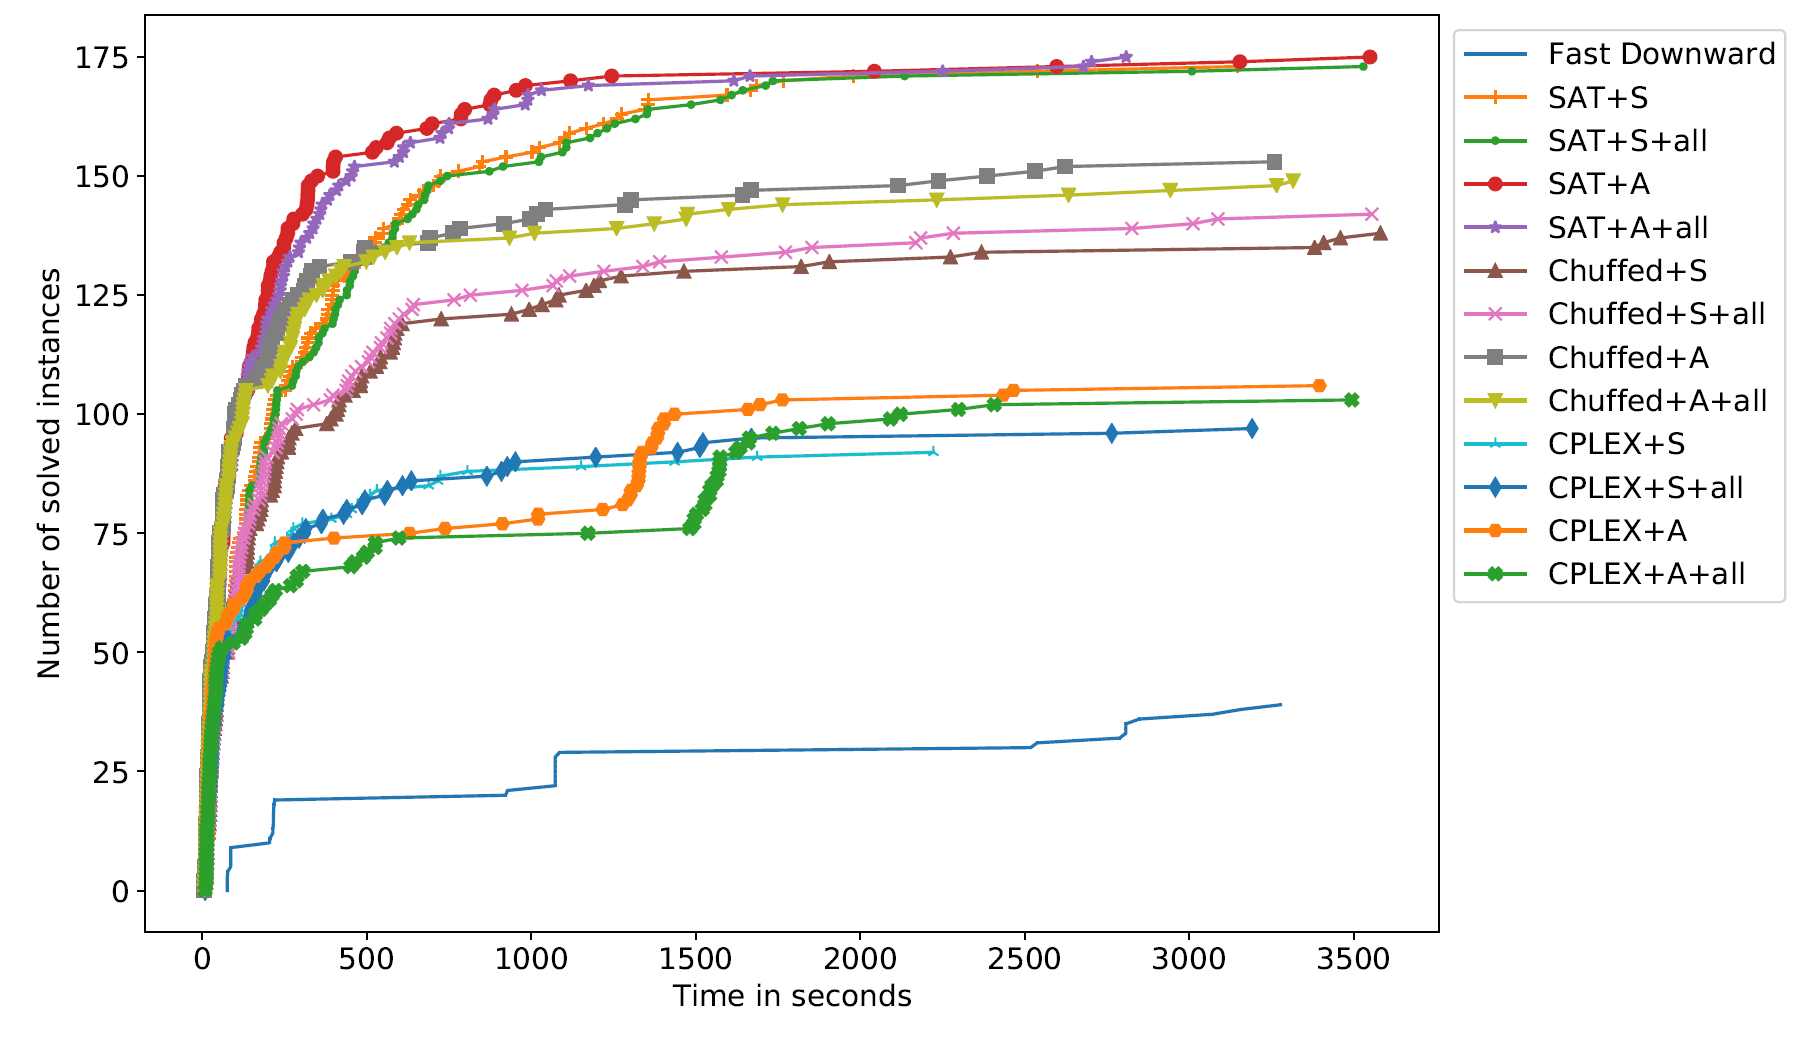
\includegraphics[width=\textwidth, height=0.3\textheight, keepaspectratio]{Images/PlottingSolverComparison.png}
    \caption{Comparing performance of Plotting models and solvers  \cite{Plotting_Planning_Problem}}
    \label{fig:plottingSolverComparison}
\end{figure}

%\subsection{Constraint Types}
%\subsubsection{Global}
%\subsubsection{Local}

\section{Wave Function Collapse}
Wave Function Collapse (WFC) \cite{Gumin_Wave_Function_Collapse_2016} is a modern PCG method that has found use in games such as Townscaper \cite{townscaper} and Bad North \cite{badnorth}. It can be described as a family of algorithms, rather than one specific algorithm \cite{WFC_ConstraintSolving_and_ML}. As such, a large variety of implementations are available online, each with their own specialisations to solve the problem they were designed for. One paper noted that Wave Function Collapse is often used as a black box, being incorporated into a workflow without being altered \cite{WFC_In_The_Wild}.

\begin{figure}[H]
    \centering
    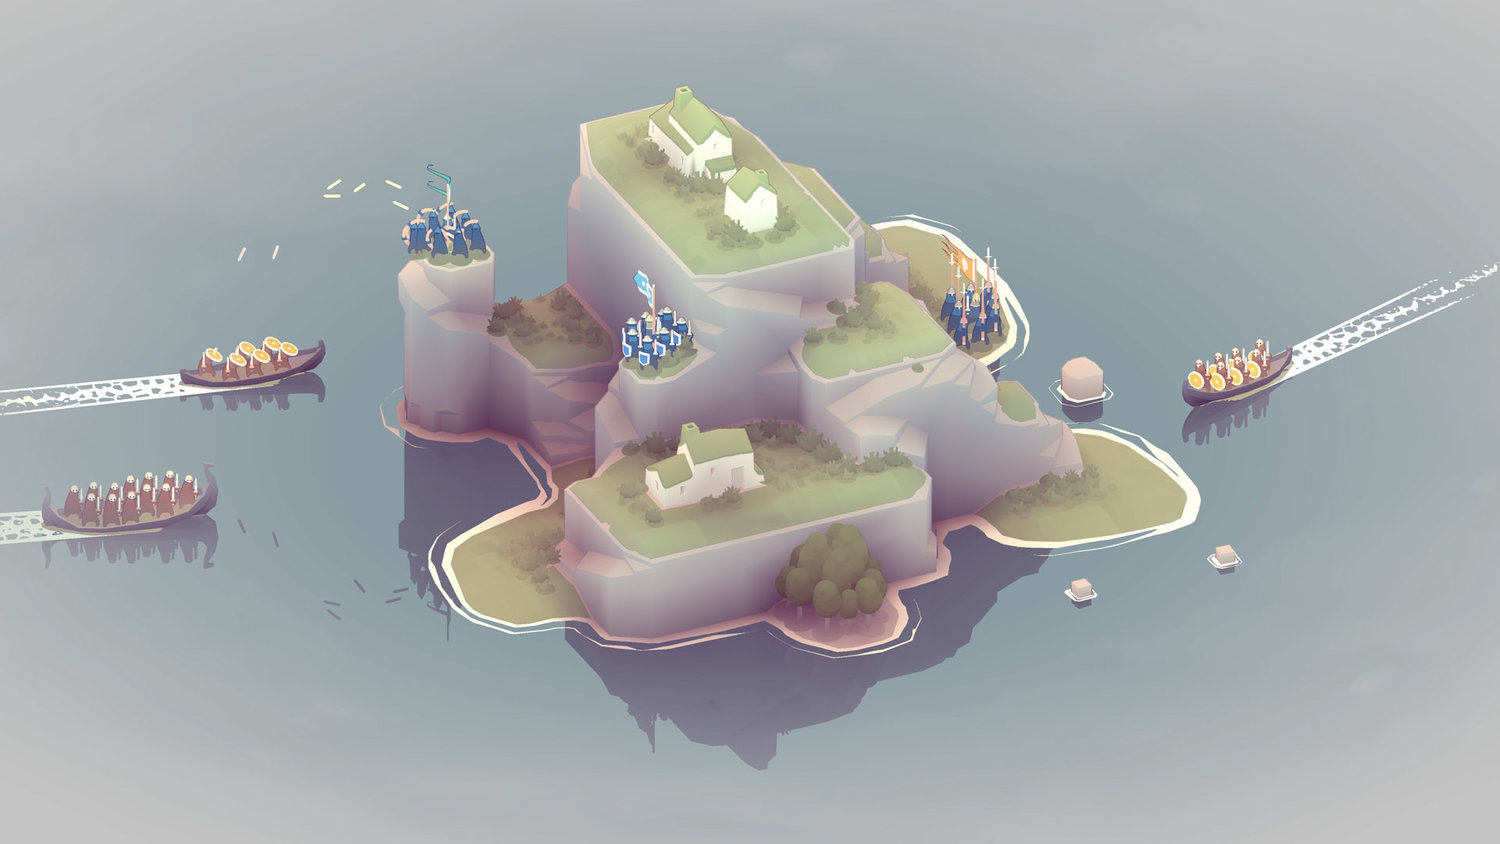
\includegraphics[width=\textwidth, height=0.3\textheight, keepaspectratio]{Images/BadNorth.jpg}
    \caption{Bad North uses WFC to generate islands traversable by AI \cite{badnorth}}
    \label{fig:badNorth}
\end{figure}

Wave Function Collapse builds off of the concepts of Model Synthesis, which is a method for procedurally modelling complex 3D shapes \cite{model_synthesis, model_synthesis_diss}. In Model Synthesis, the user defines an input model detailing various dimensional, geometric and algebraic constraints. This is then used to create output satisfying the modelled constraints. A simple example using a pillar model is shown in Figure \ref{fig:modelSynthesis}.

\begin{figure}[H]
    \centering
    \subfigure[An input model with model pieces arranged and labelled 0 to 3]{
        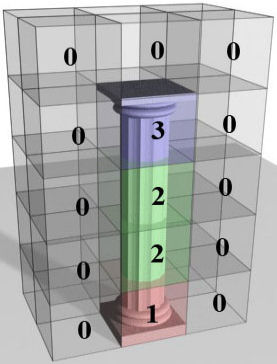
\includegraphics[width=0.475\textwidth, height=0.35\textheight, keepaspectratio]{Images/ModelSynthesis1.jpg}
        \label{fig:modelSynthesis1}
    }
    \hfill
    \subfigure[Pillar variations using the input model pieces]{
        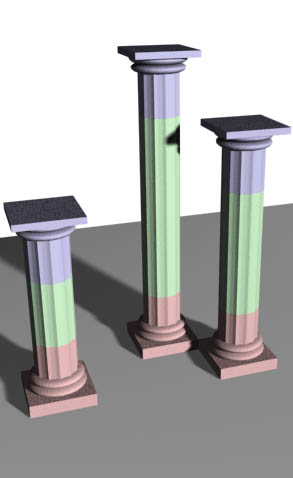
\includegraphics[width=0.475\textwidth, height=0.35\textheight, keepaspectratio]{Images/ModelSynthesis2.jpg}
        \label{fig:modelSynthesis2}
    }
    \caption{Generating pillars of different lengths from input model pieces \cite{model_synthesis_diss}}
    \label{fig:modelSynthesis}
\end{figure}

\subsection{Implementation Variations}
\subsubsection{Data Input}
The data input stage is likely the WFC stage with the most variation across implementations. The original implementation \cite{Gumin_Wave_Function_Collapse_2016} supports both an overlapping and simple tiled model. The overlapping version takes a sample image and defines overlapping patterns of \(N\times N\) tiles, where the output is constructed of a random arrangement of these patterns. The overlapping WFC pipeline is shown in Figure \ref{fig:overlappingWFC}. The simple tiled model instead defines single tile patterns, where each tile has its own defined set of possible neighbours. An example of simple tiled generation was shown in the Introduction in Figure \ref{fig:WFCcircuit}.

\begin{figure}[H]
    \centering
    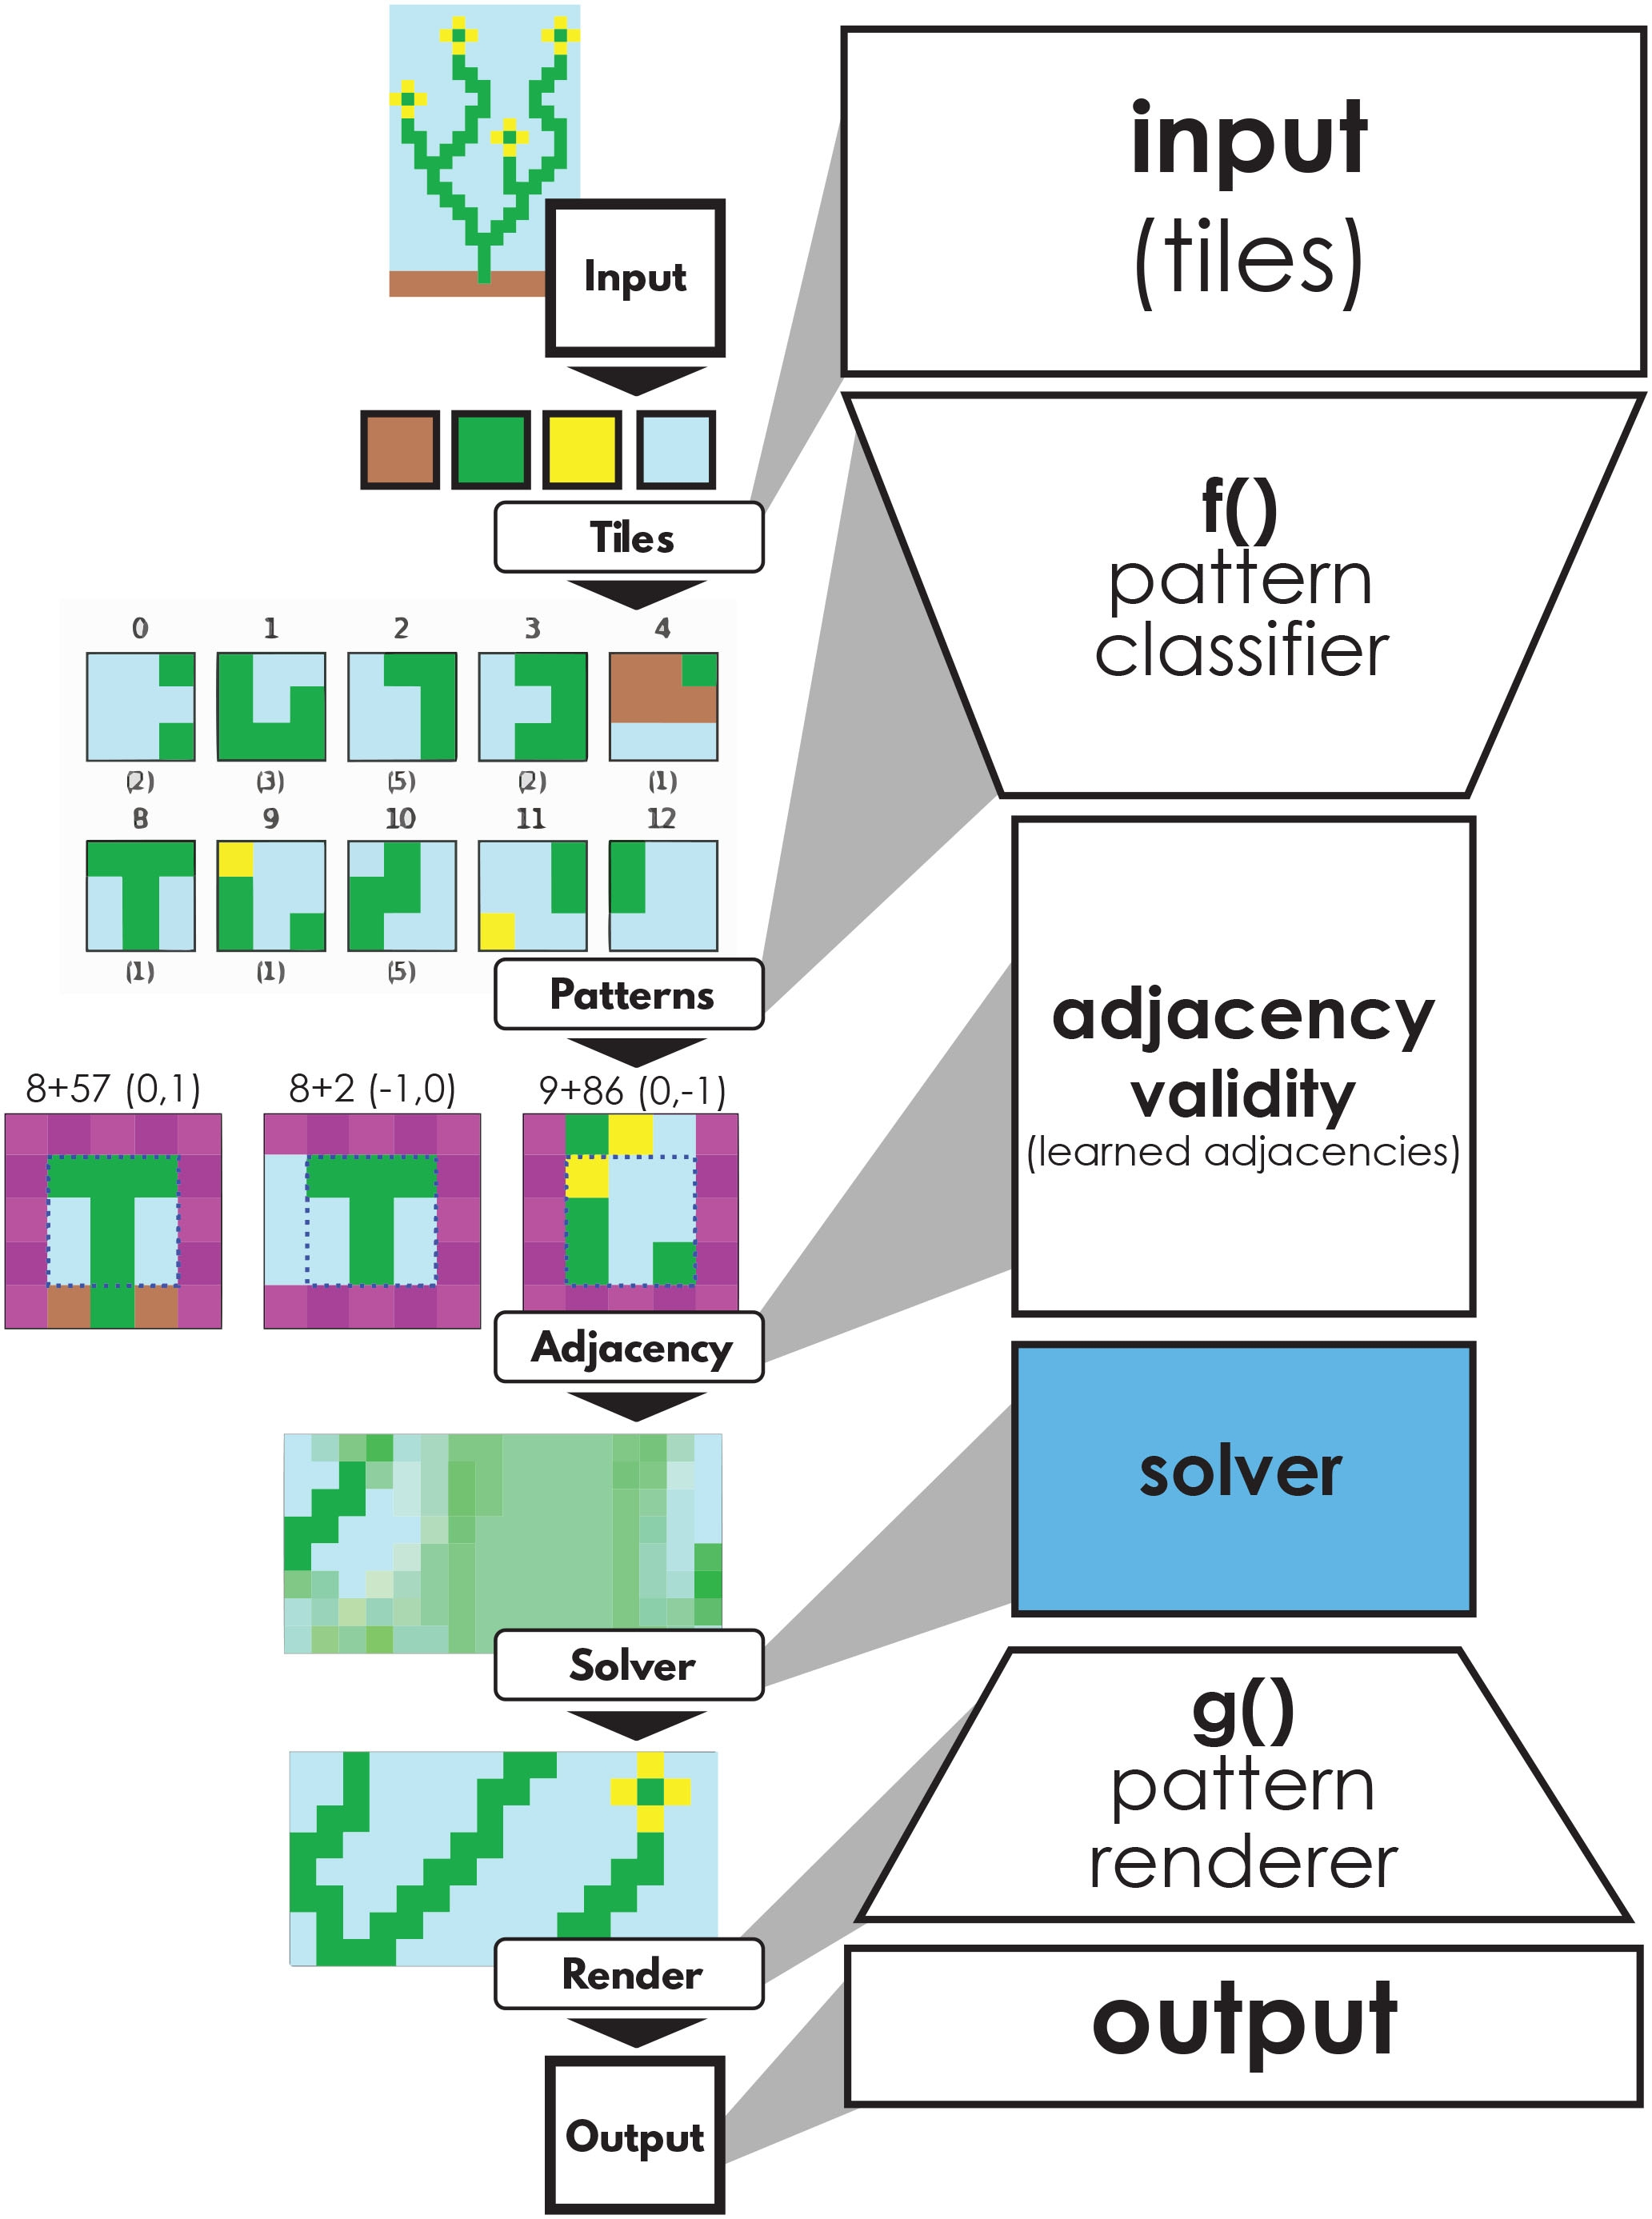
\includegraphics[width=\textwidth, height=0.5\textheight, keepaspectratio]{Images/OverlappingWFC.jpg}
    \caption{The overlapping WFC pipeline with \(3\times 3\) overlap \cite{WFC_ConstraintSolving_and_ML}}
    \label{fig:overlappingWFC}
\end{figure}

\subsubsection{2D vs 3D}
While a lot of implementations focus solely on 2D input tiles and grids, much fewer implementations support 3D input or output. This makes it a challenge to apply WFC to 3D environments. Furthermore, the increased complexity from a 3D environment can lead to an increased failure rate, which requires techniques such as backtracking or modifying in blocks to counteract. This was highlighted in the Introduction with Figure \ref{fig:escheresque}.

\subsection{Limitations of Wave Function Collapse}
Research papers on WFC frequently attempt to identify and find solutions for problems that implementations of the algorithm commonly face. Some of the most common problems are a lack of global constraints, overfitting and performance. These problems, as well as some other challenges, are discussed below.

%\begin{itemize}
%\item Isotropy / Homogeneity: Without global constraints there is no inherent overall structure.
%\item Overfitting: Adding too much detail to input or using too high overlapping can result in the input being copied directly too much.
%\item Performance: Slower than model synthesis [17]? Is this due to additional checks like lowest entropy vs scanning?
%\item Contradictions / Failures: Has a tendency to fail for big inputs, especially in 3D.
%\end{itemize}

\subsubsection{Lack of Global Constraints}
One problem with WFC is that, while output can be tailored to satisfy local constraints, global constraints are not inherently supported. This results in there being no inherent overall structure to the output. In other words, the output can be homogeneous.

In some applications, such as the game Caves of Qud \cite{cavesofqud}, WFC is used only after other algorithms have defined distinct regions of the map as shown in Figure \ref{fig:cavesOfQudWFCHomogeneity} \cite{WFC_ConstraintSolving_and_ML, WFC_Design_Constraints, GDC_caves_of_qud}. This multi-pass approach allows WFC to be used to its strengths.

\begin{figure}[H]
    \centering
    \subfigure[Areas of the level set before using WFC]{
        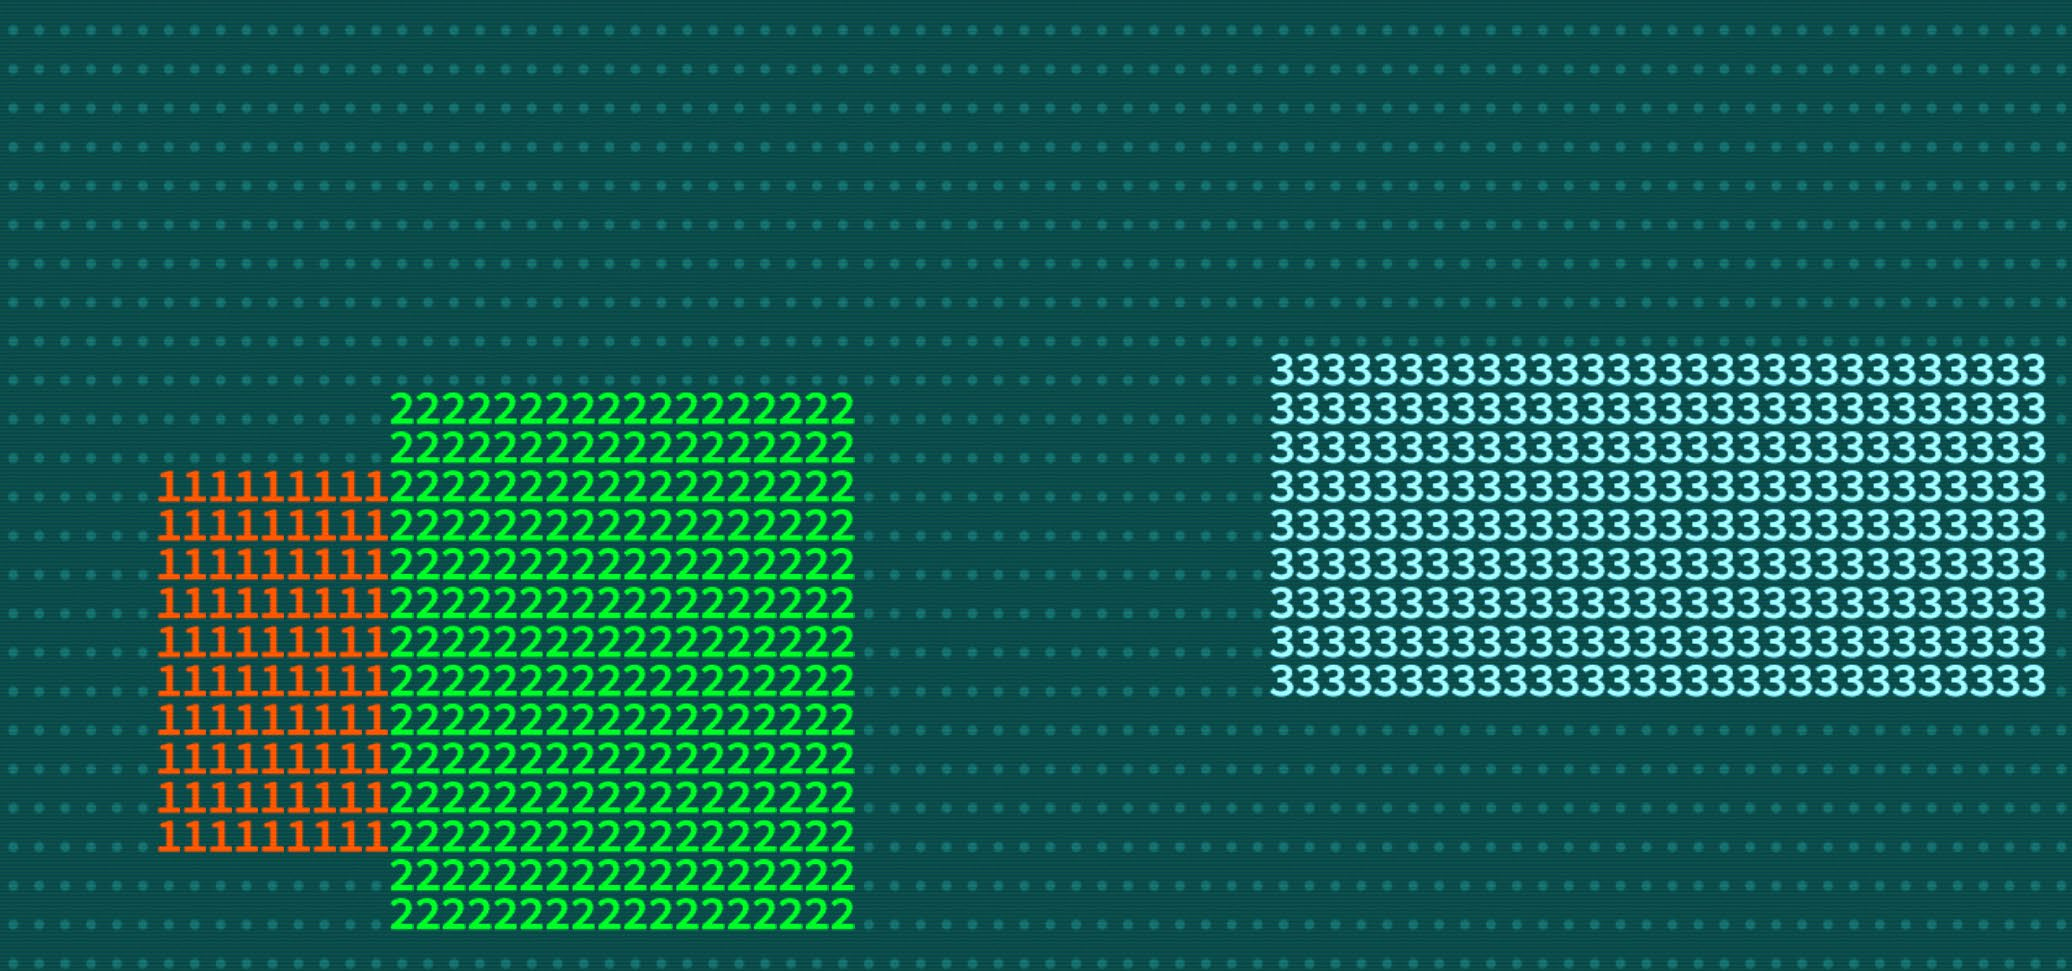
\includegraphics[width=0.475\textwidth, height=0.35\textheight, keepaspectratio]{Images/CavesOfQudWFC1.jpg}
        \label{fig:cavesOfQudWFC1}
    }
    \hfill
    \subfigure[Interiors generated using WFC]{
        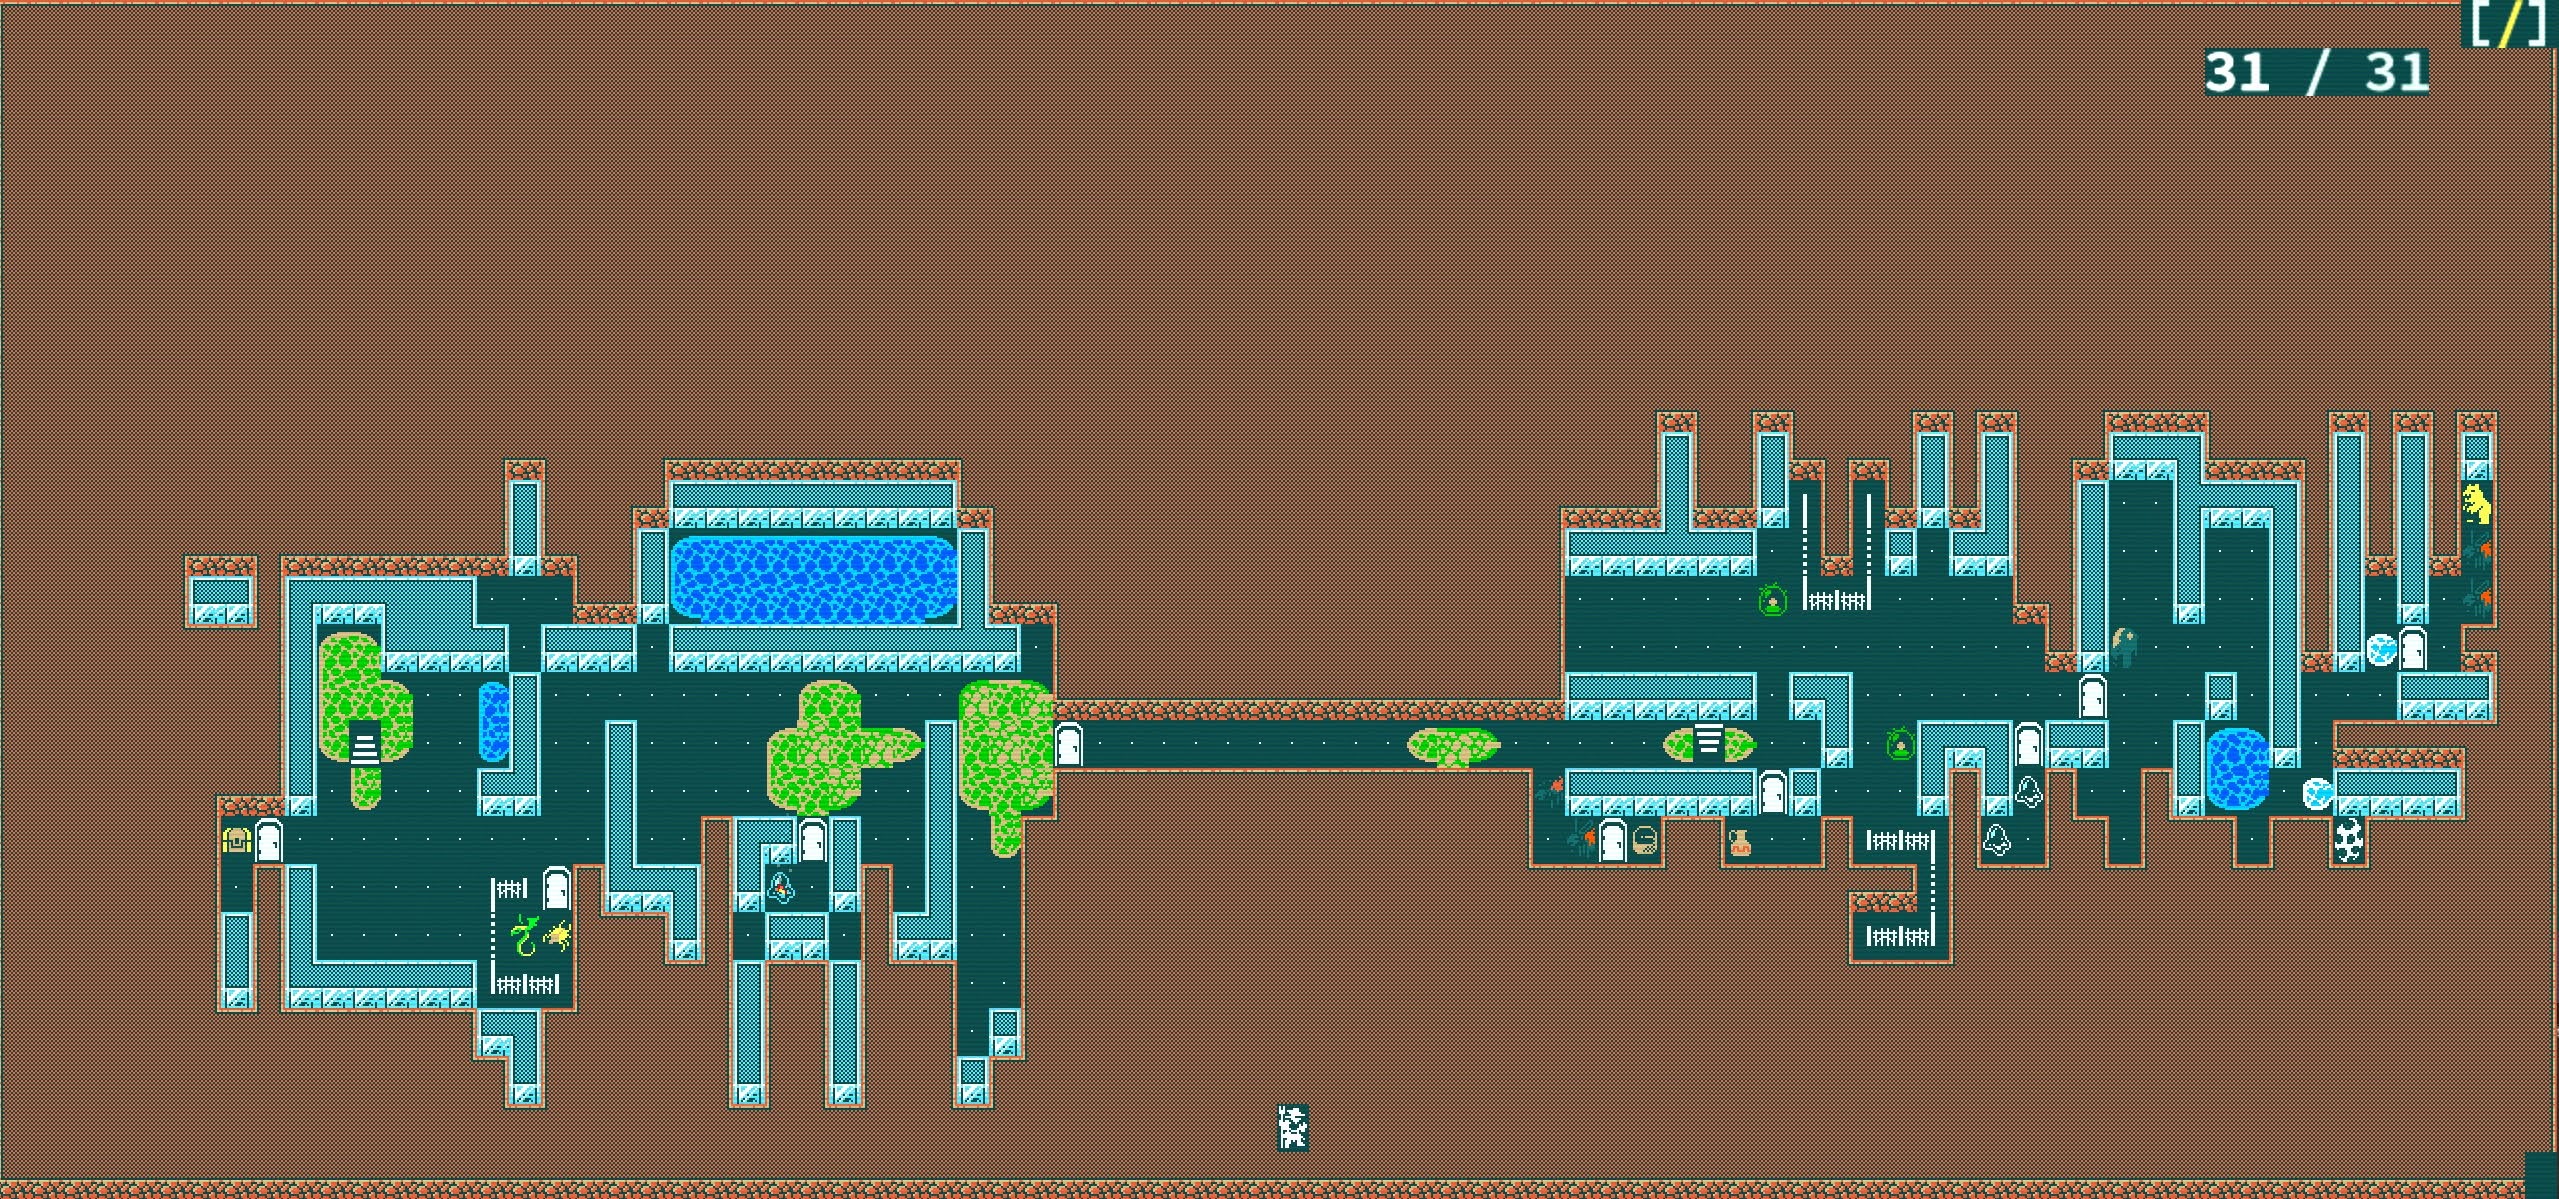
\includegraphics[width=0.475\textwidth, height=0.35\textheight, keepaspectratio]{Images/CavesOfQudWFC2.jpg}
        \label{fig:cavesOfQudWFC2}
    }
    \caption{Caves of Qud's multi-pass approach to avoid homogeneity \cite{GDC_caves_of_qud}}
    \label{fig:cavesOfQudWFCHomogeneity}
\end{figure}

Two papers add in additional constraints that are checked after each observation step. In the first paper \cite{WFC_Automatic_Rules_And_Better_Symmetries}, constraints added include a minimum tile count, maximum tile count and object distance constraint.

The global maximum tile count constraint allows balancing of tile counts. This constraint is analogous to the use of weighted tile selection. Figure \ref{fig:wfcMaximumConstraint} shows the global maximum tile count constraint being used to reduce the amount of water in the level.

\begin{figure}[H]
    \centering
    \subfigure[Generation without the maximum constraint]{
        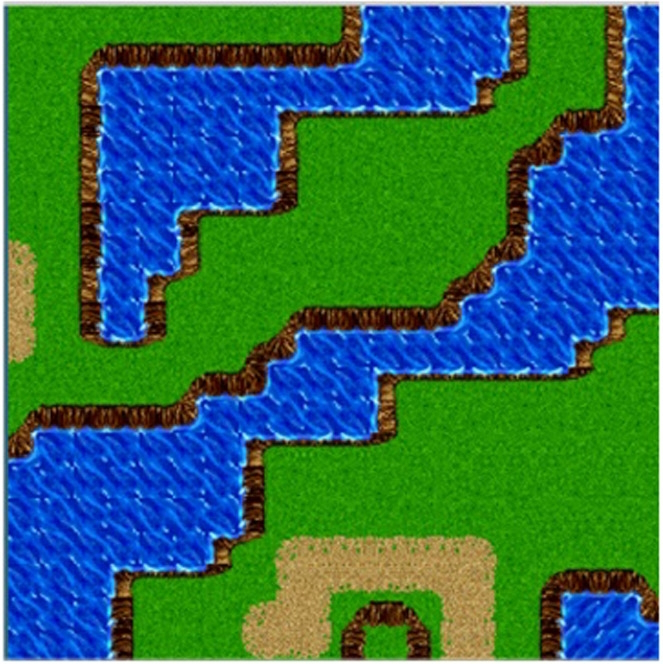
\includegraphics[width=0.475\textwidth, height=0.35\textheight, keepaspectratio]{Images/WFCMaximumConstraint1.jpg}
        \label{fig:wfcMaximumConstraint1}
    }
    \hfill
    \subfigure[Generation with the maximum constraint]{
        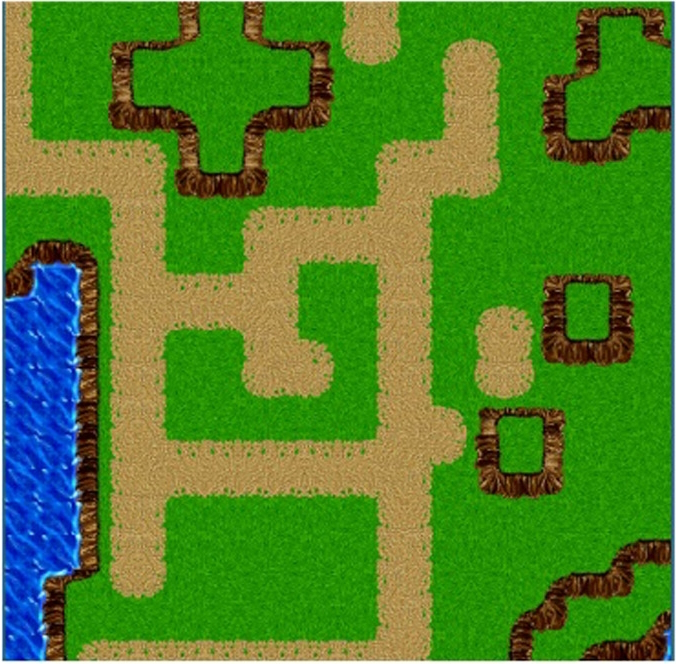
\includegraphics[width=0.475\textwidth, height=0.35\textheight, keepaspectratio]{Images/WFCMaximumConstraint2.jpg}
        \label{fig:wfcMaximumConstraint2}
    }
    \caption{Use of the global maximum constraint to limit water tiles \cite{WFC_Automatic_Rules_And_Better_Symmetries}}
    \label{fig:wfcMaximumConstraint}
\end{figure}

The global minimum tile count constraint gives more control on how tiles should be placed in the level. The way it is presented in the paper shows it being used to preset tiles before generation. This enables the definition of key areas that should be present in the output. Figure \ref{fig:wfcMinimumConstraint} shows the global minimum tile count constraint being used to place water in the bottom left and land in the middle of the level.

\begin{figure}[H]
    \centering
    \subfigure[Pre-setting water and land tiles]{
        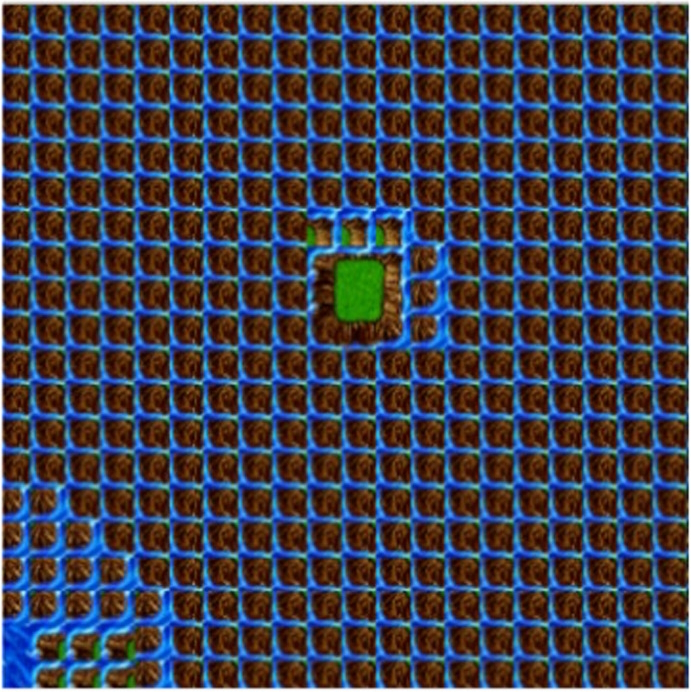
\includegraphics[width=0.475\textwidth, height=0.35\textheight, keepaspectratio]{Images/WFCMinimumConstraint1.jpg}
        \label{fig:wfcMinimumConstraint1}
    }
    \hfill
    \subfigure[Generation with the minimum constraint]{
        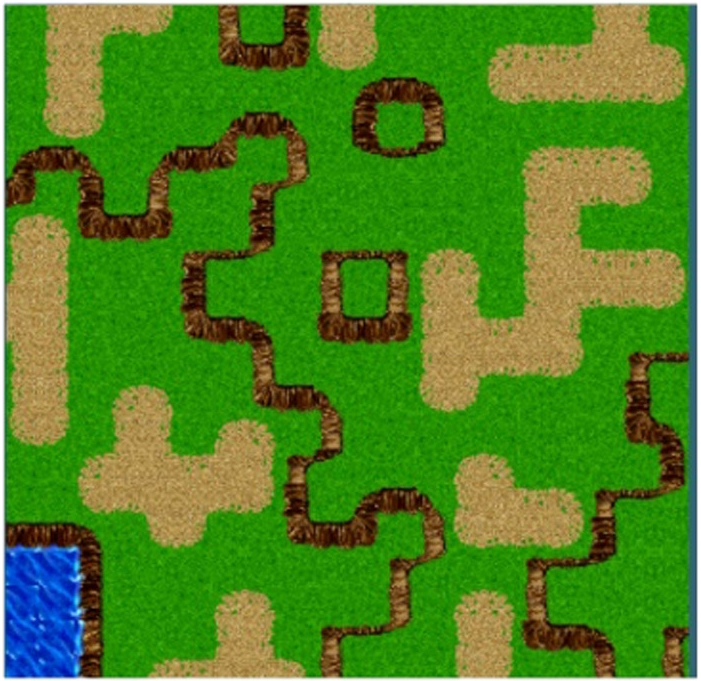
\includegraphics[width=0.475\textwidth, height=0.35\textheight, keepaspectratio]{Images/WFCMinimumConstraint2.jpg}
        \label{fig:wfcMinimumConstraint2}
    }
    \caption{Use of the global minimum constraint to pre-place tiles \cite{WFC_Automatic_Rules_And_Better_Symmetries}}
    \label{fig:wfcMinimumConstraint}
\end{figure}

The object distance constraint is used to create areas of interest, rather than scattering items equally throughout the level. Figure \ref{fig:wfcDistanceConstraint1} shows how without an object distance constraint, enemies and items are scattered at random throughout the level. In contrast, Figure \ref{fig:wfcDistanceConstraint2} shows how enemies are clustered around a treasure chest. To achieve this, enemies are constrained to be less than 10 units away from chests. Furthermore, keys are constrained to be more than 10 units away from chests. This means that keys will not simply spawn next to chests, making finding them more interesting.

\begin{figure}[H]
    \centering
    \subfigure[Generation without the distance constraint]{
        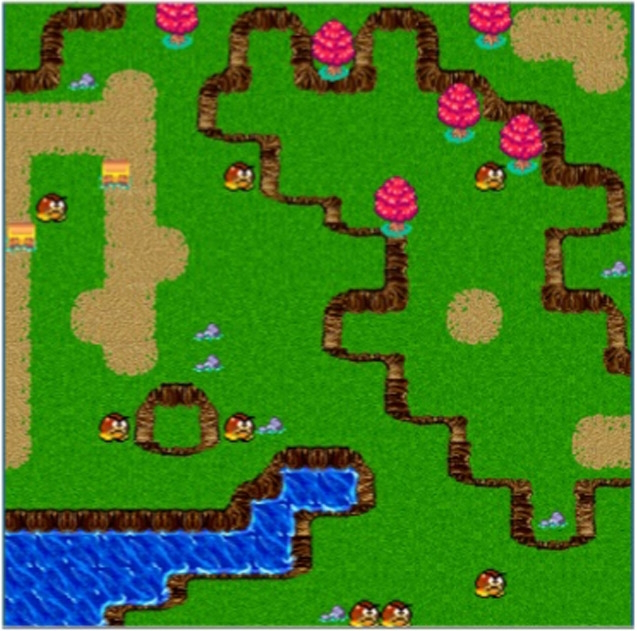
\includegraphics[width=0.475\textwidth, height=0.35\textheight, keepaspectratio]{Images/WFCDistanceConstraint1.jpg}
        \label{fig:wfcDistanceConstraint1}
    }
    \hfill
    \subfigure[Generation with the distance constraint]{
        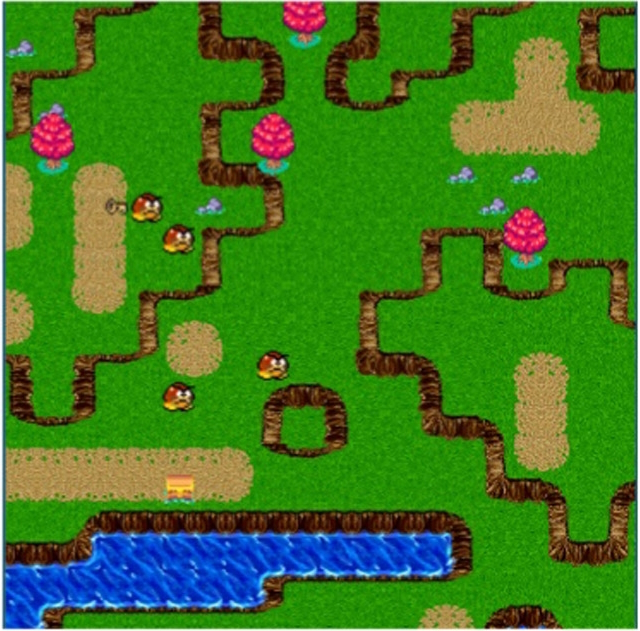
\includegraphics[width=0.475\textwidth, height=0.35\textheight, keepaspectratio]{Images/WFCDistanceConstraint2.jpg}
        \label{fig:wfcDistanceConstraint2}
    }
    \caption{Use of the object distance constraint to improve object spawns \cite{WFC_Automatic_Rules_And_Better_Symmetries}}
    \label{fig:wfcDistanceConstraint}
\end{figure}

One additional option included is to carry out generation in two passes. This helps create levels of certain styles and to reduce conflicts arising from trying to generate everything in one pass, such as placing an object on an unsuitable tile. In Figure \ref{fig:wfcMultiLayer}, double-layer generation is used to spawn enemies on grass and chests on dirt roads. Furthermore, rock and dirt decor is placed on suitable tiles.

\begin{figure}[H]
    \centering
    \subfigure[Single-layer generation]{
        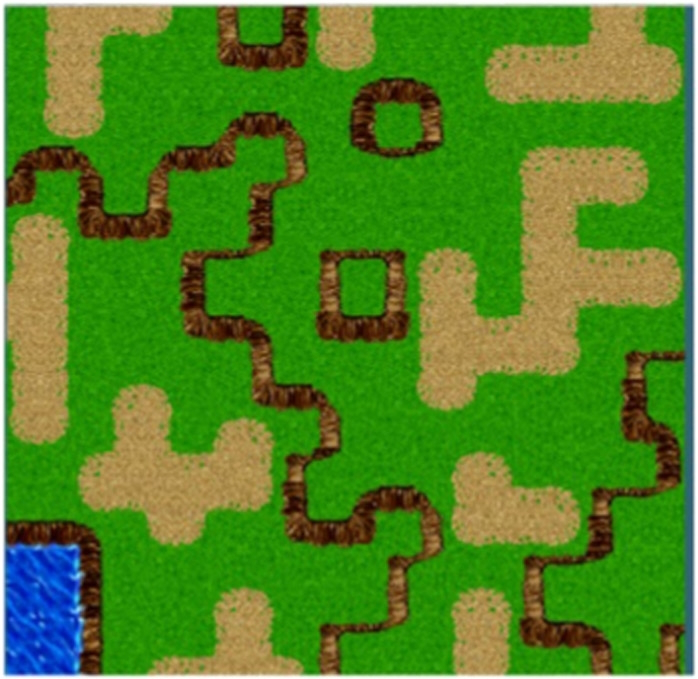
\includegraphics[width=0.475\textwidth, height=0.35\textheight, keepaspectratio]{Images/WFCMultiLayer1.jpg}
        \label{fig:wfcMultiLayer1}
    }
    \hfill
    \subfigure[Double-layer generation]{
        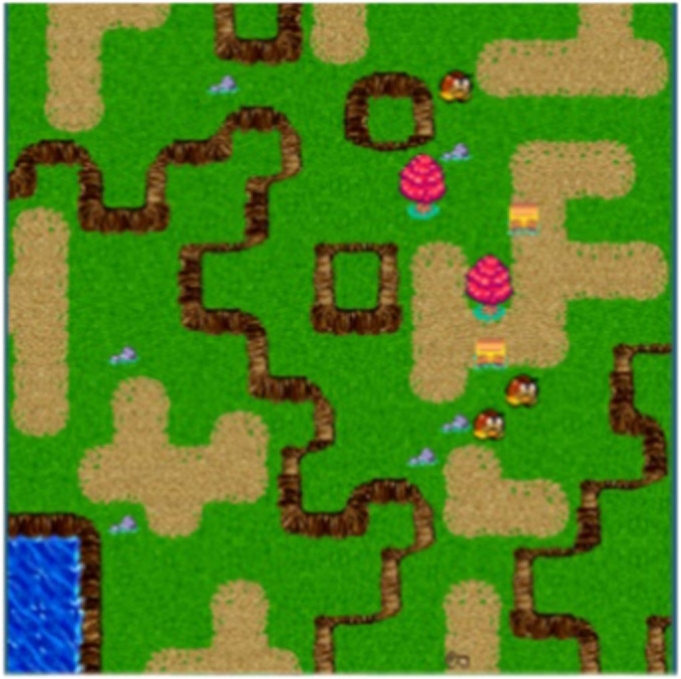
\includegraphics[width=0.475\textwidth, height=0.35\textheight, keepaspectratio]{Images/WFCMultiLayer2.jpg}
        \label{fig:wfcMultiLayer2}
    }
    \caption{Use of the double-layer generation to ease object spawning \cite{WFC_Automatic_Rules_And_Better_Symmetries}}
    \label{fig:wfcMultiLayer}
\end{figure}

The second paper, \cite{WFC_Design_Constraints}, achieves the same goal as minimum and maximum tile count constraints through the use of a weighted choice. In addition to using entropy to choose the most constrained tile after each propagation step, assigning a weight to each choice can encourage the algorithm to choose a different balance of tiles. Furthermore, this paper introduces a second observation step. This performs a second, smaller scale WFC algorithm, which can be used to refine item placement and create subregions within a map.

Solutions altering WFC directly to support global constraints are faced with the issue that the additional constraints can have a negative impact on performance. However, by combining such solutions with those discussed in the Performance Subsection (\ref{sec:performance}), the impact can be reduced \cite{WFC_ConstraintSolving_and_ML}.

\subsubsection{Overfitting}
When adding a lot of detail to the input, such as through using complex tile sets, the output may become too constrained. This can result in overfitting and an increased failure rate.

Here, a multi-pass approach can not only be used to help globally constrain the output, but also to reduce risk of overfitting. This is done by reducing the detail of the input and instead adding additional details to the output in a second pass once WFC has run. Caves of Qud applies this approach by generating architecture using WFC and then generating details using additional passes as in Figure \ref{fig:cavesOfQudWFCOverfitting} \cite{GDC_caves_of_qud}.

\begin{figure}[H]
    \centering
    \subfigure[Architecture generated using WFC]{
        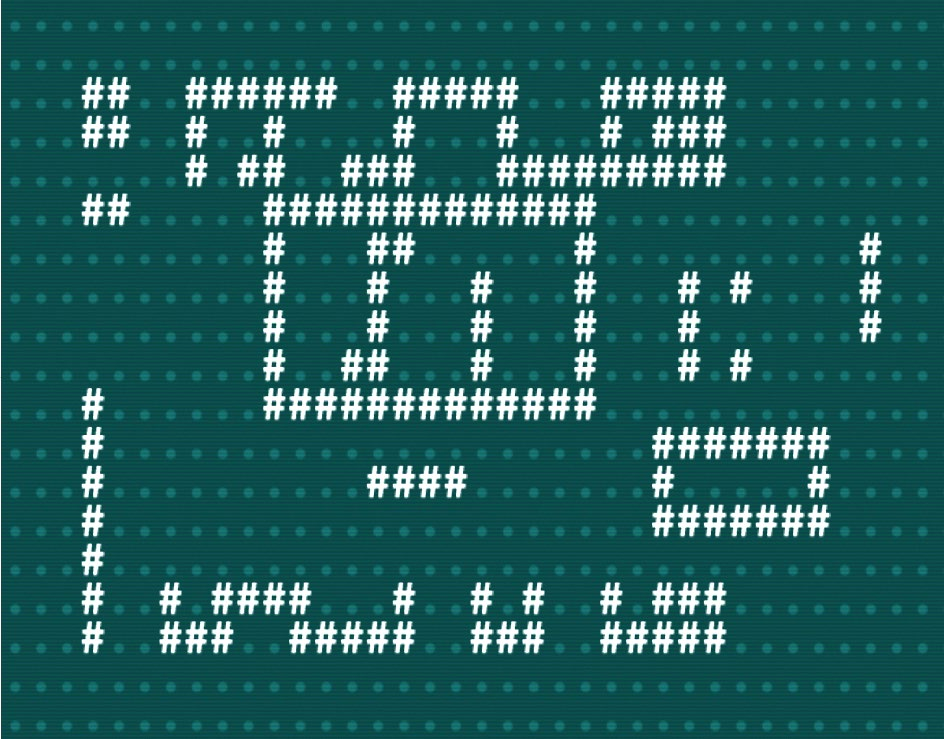
\includegraphics[width=0.475\textwidth, height=0.35\textheight, keepaspectratio]{Images/CavesOfQudWFC3.jpg}
        \label{fig:cavesOfQudWFC3}
    }
    \hfill
    \subfigure[Details filled using additional passes]{
        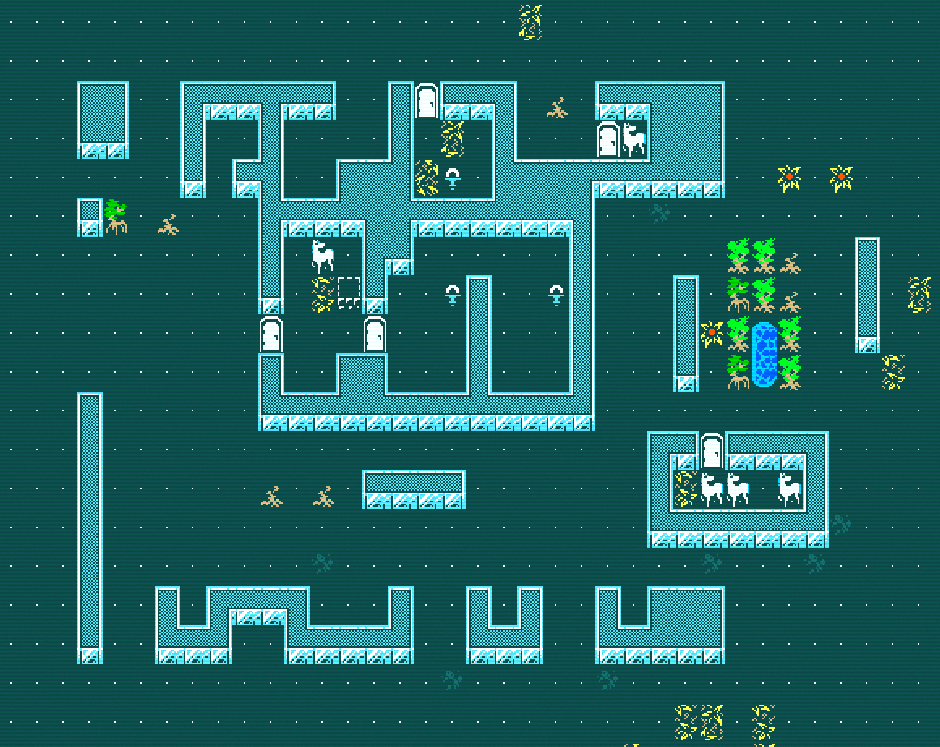
\includegraphics[width=0.475\textwidth, height=0.35\textheight, keepaspectratio]{Images/CavesOfQudWFC4.png}
        \label{fig:cavesOfQudWFC4}
    }
    \caption{Caves of Qud's multi-pass approach to avoid overfitting \cite{GDC_caves_of_qud}}
    \label{fig:cavesOfQudWFCOverfitting}
\end{figure}

%Furthermore, when using the overlapping method for WFC, a high overlap parameter will also result in overfitting. This may be difficult to balance depending on the input.

\subsubsection{Performance}\label{sec:performance}
Another issue identified with WFC is performance. While the chance of success is high with small inputs, larger inputs are much likelier to fail, especially with more complicated tile sets \cite{WFC_ConstraintSolving_and_ML}. This can result in a significant generation time for large outputs. Several solutions to WFC's scalability problem have been proposed.%(More citations and graph of performance)

One of the most common solutions is to include some form of backtracking, which allows further searching of the search space upon a contradiction instead of having to restart. However, with complex tile sets, care must be taken to reduce the chance of backtracking exploring an unpromising search space for an extended time as in the 3D Escheresque example shown previously in Figure \ref{fig:escheresque}. Using a search heuristic could help with this. One paper compared the performance of WFC with and without backtracking and global constraints, finding that backtracking is critical to improving performance when using global constraints as seen in Figure \ref{fig:backtrackingPerformance} \cite{WFC_ConstraintSolving_and_ML}.

\begin{figure}[H]
    \centering
    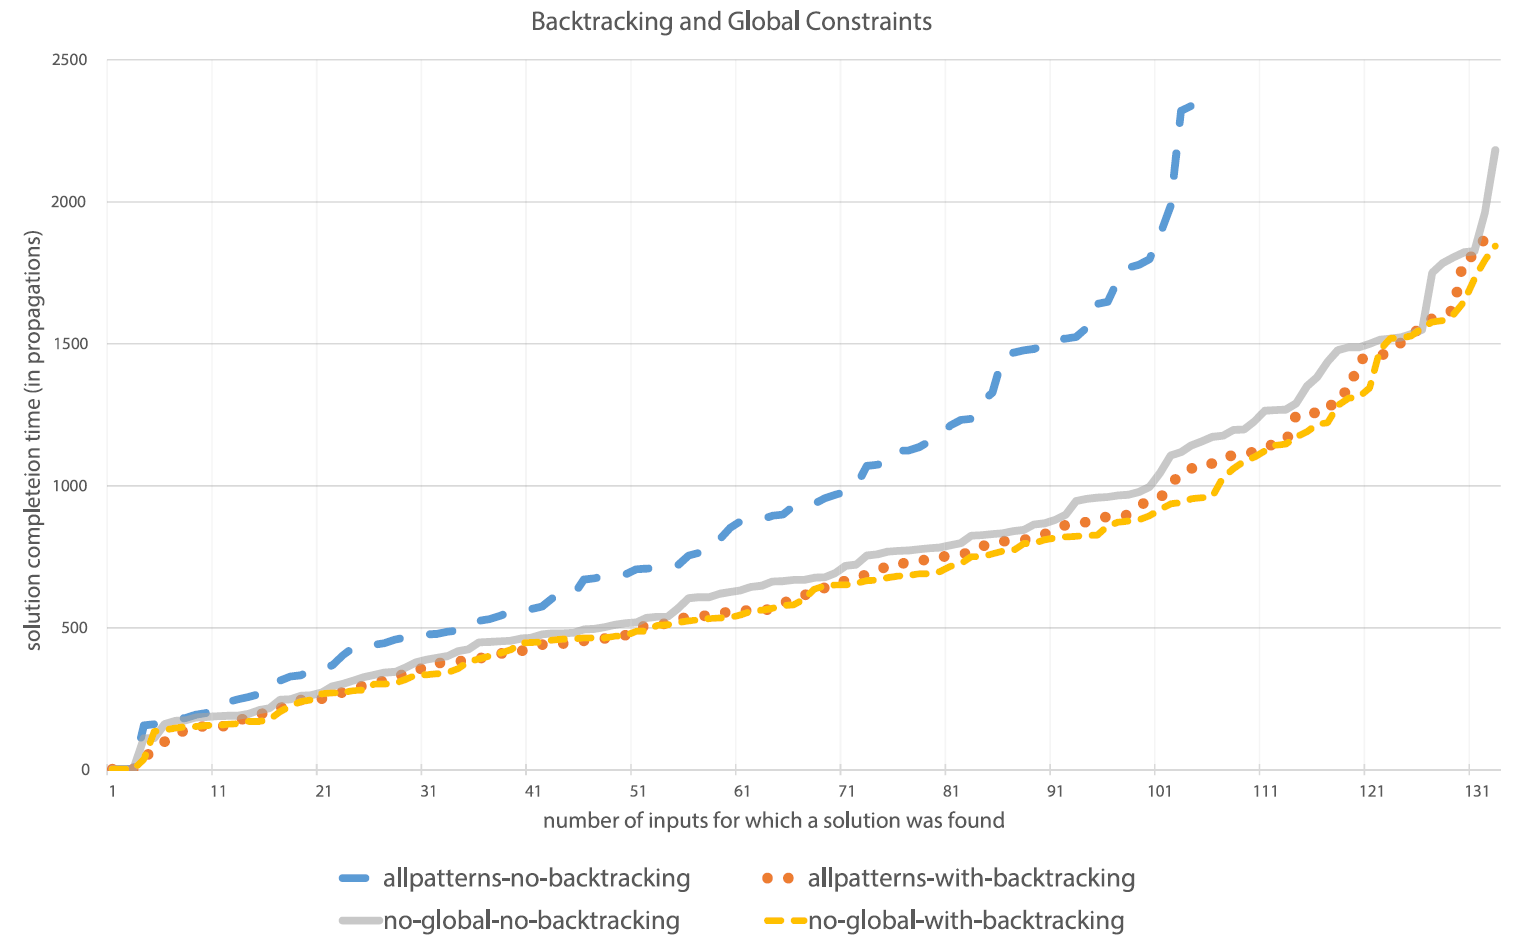
\includegraphics[width=\textwidth, height=0.3\textheight, keepaspectratio]{Images/BacktrackingPerformance.png}
    \caption{Comparing performance of WFC with and without backtracking and global constraints. When using global constraints, backtracking significantly improves performance. \cite{WFC_ConstraintSolving_and_ML}}
    \label{fig:backtrackingPerformance}
\end{figure}

Nested WFC (N-WFC) \cite{Nested_WFC} is one technique that aims to improve scalability of WFC. It splits a larger grid into smaller grids, evaluating sub-grids diagonally from the top left as in Figure \ref{fig:nestedWFC}. Each sub-grid overlaps constraints from its left and upper neighbour to satisfy constraints between adjacent sub-grids. This can be extended to an infinite space by overlapping new cells with old cells as in Figure \ref{fig:infiniteWFC}. While this technique does improve the performance of WFC, evaluation found that that a large number of conflicts from edge data still occur.

\begin{figure}[H]
    \centering
    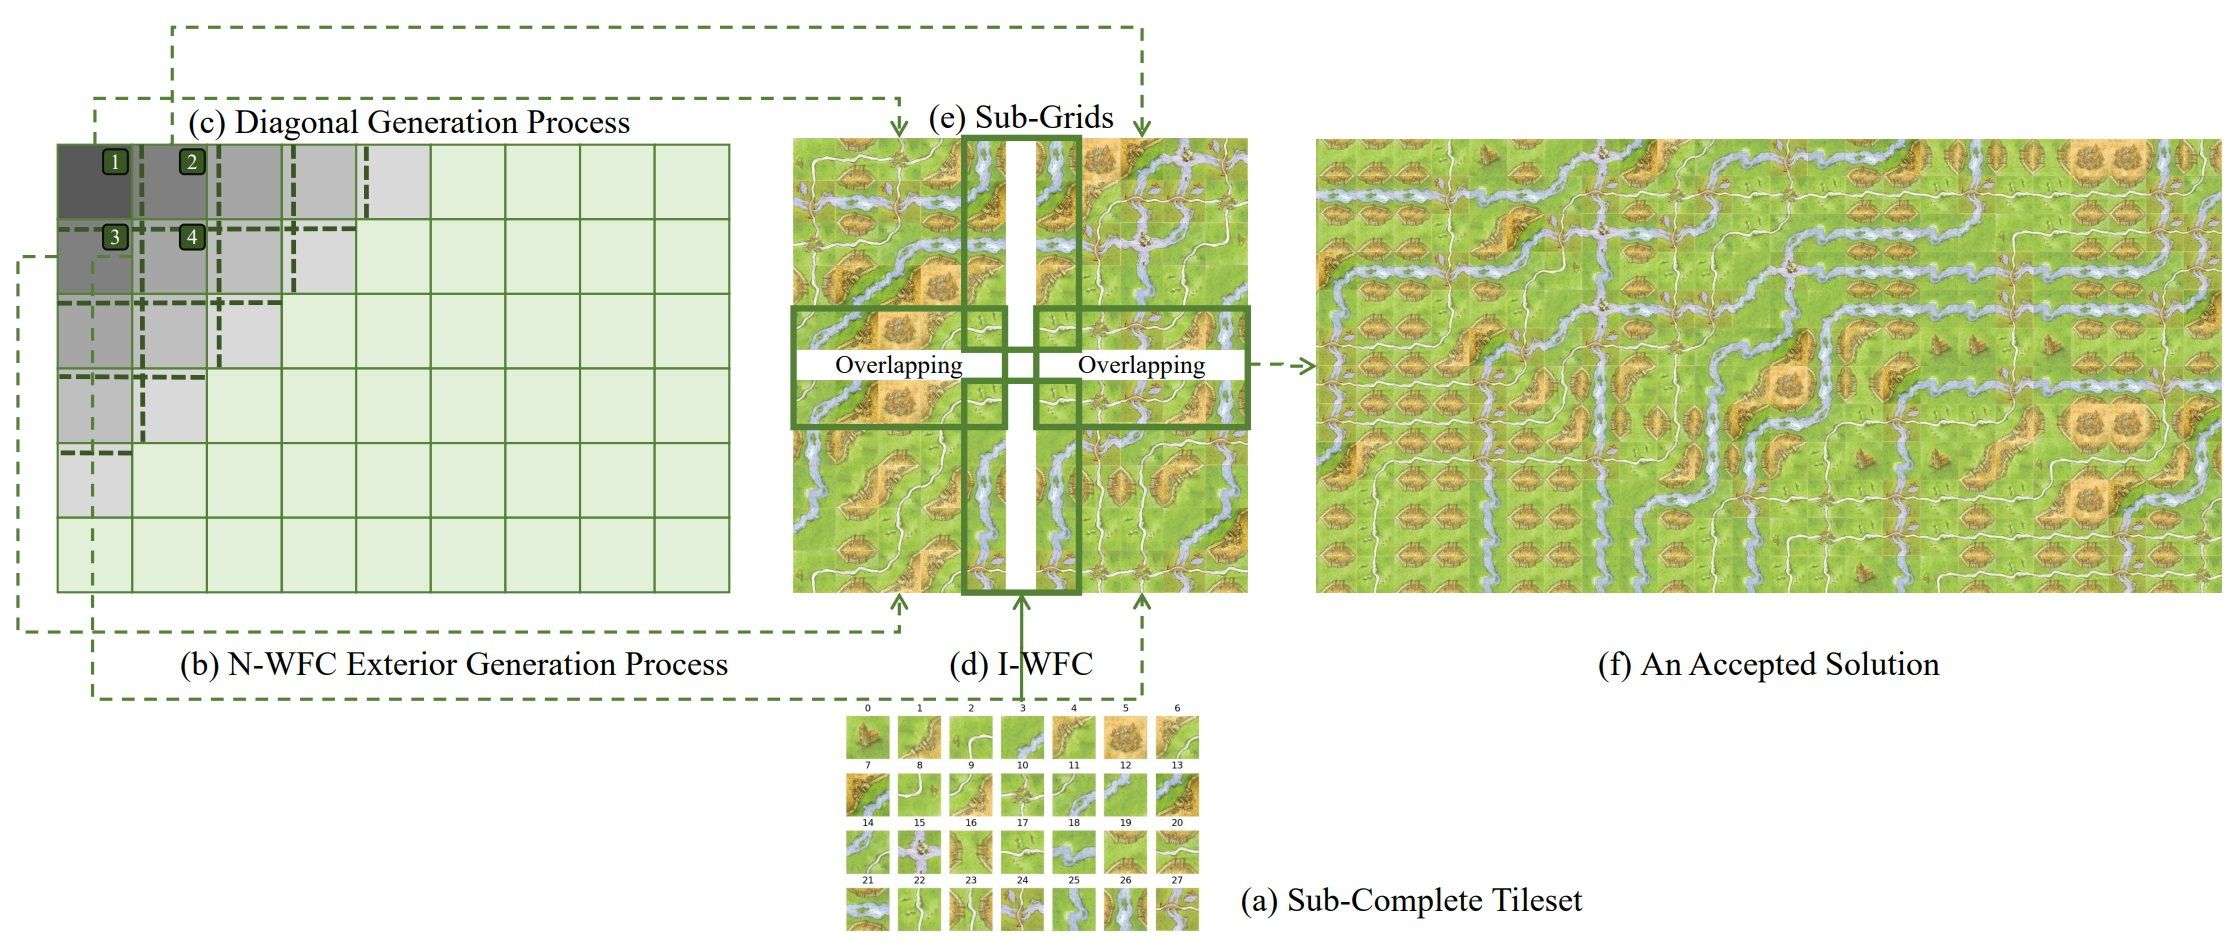
\includegraphics[width=\textwidth, height=0.3\textheight, keepaspectratio]{Images/NestedWFC.jpg}
    \caption{Large-scale game implementation with N-WFC and sub-complete tile set. First, it requires (a) one sub-complete tile set. Then the (b) Exterior Generation Process uses (c) Diagonal Generation Process to start generating. Each (d) sub-grid uses (e) I-WFC to find an accepted solution and overlap its edge with the adjacent sub-grids, forming an (f) final soluton. \cite{Nested_WFC}}
    \label{fig:nestedWFC}
\end{figure}

\begin{figure}[H]
    \centering
    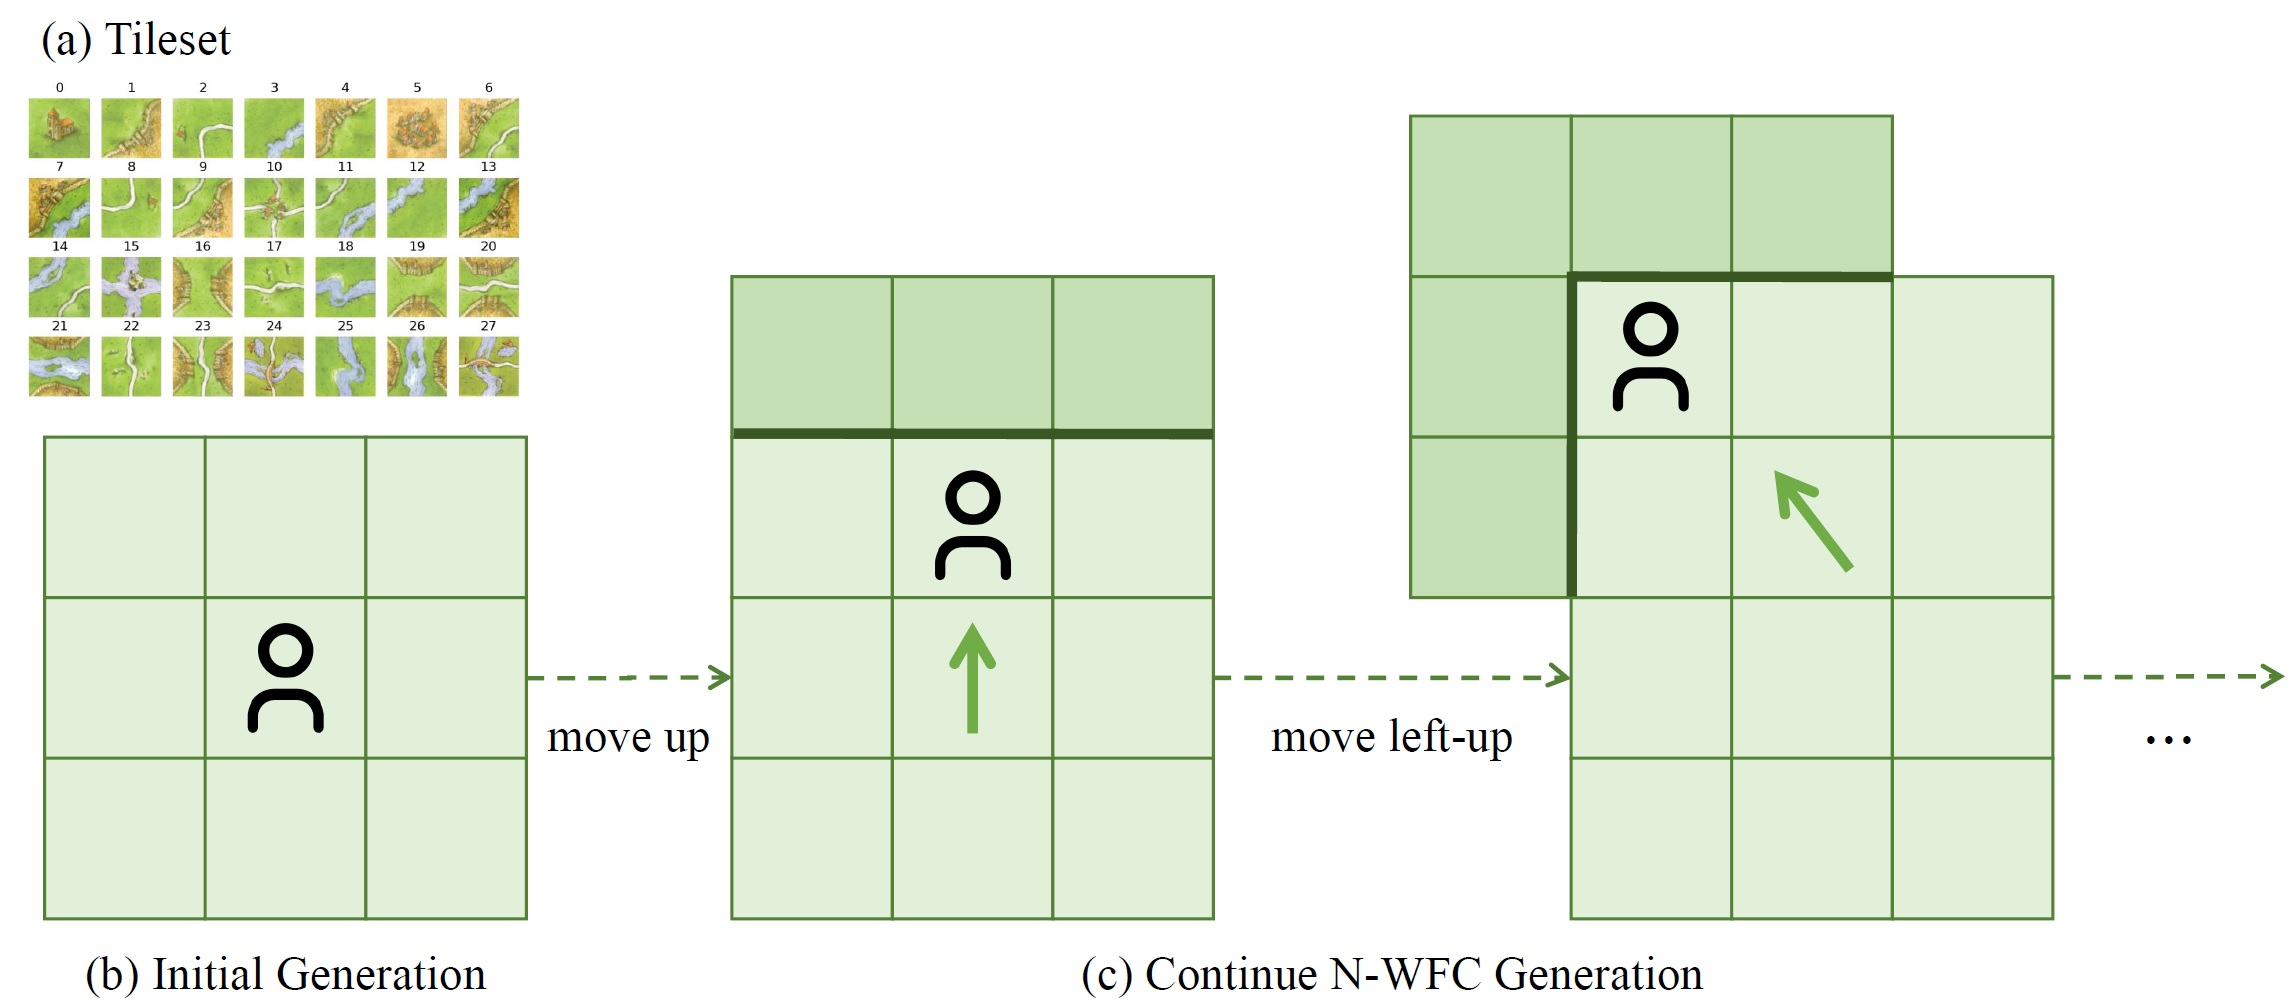
\includegraphics[width=\textwidth, height=0.3\textheight, keepaspectratio]{Images/InfiniteWFC.jpg}
    \caption{Infinite game implementation with N-WFC and sub-complete tile set \cite{Nested_WFC}}
    \label{fig:infiniteWFC}
\end{figure}

Another technique, infinite modifying in blocks \cite{Infinite_Modifying_In_Blocks}, applies WFC multiple times in small chunks. Keeping the chunks small keeps the performance of generation high, while running WFC in four layers per chunk ensures that constraints are satisfied between adjacent chunks. The layering also addresses the limitation of conflicts that Nested WFC struggles with. As each chunk is made up of four WFC layers, failed layers can usually be ignored rather than having to be regenerated. However, this comes with computational overhead from running WFC four times per chunk. An overview of the method was shown in Figure \ref{fig:imib}.

\subsubsection{Other Challenges}
Environments of a certain style, especially those trying to create a realistic feel, may struggle from WFC's use of a grid structure for its output. However, if this regular grid is transformed into an irregular quadrilateral grid, more complex shapes can be used.

One paper \cite{WFC_Graph-based} achieves this by using a graph-based data structure, which can be integrated with a navigation mesh in 3D as shown in Figure \ref{fig:navigationMeshNodePlacement}. However, this solution is limited due to a lack of control over solution order.

\begin{figure}[H]
    \centering
    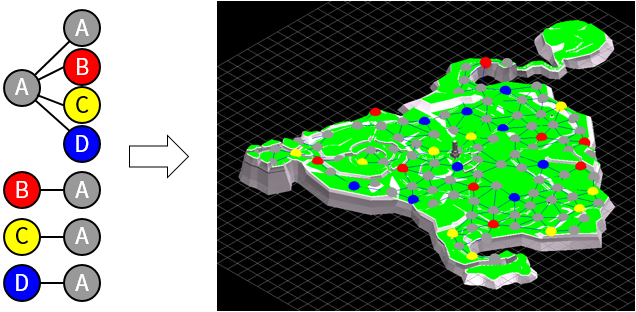
\includegraphics[width=\textwidth, height=0.3\textheight, keepaspectratio]{Images/NavigationMeshNodePlacement.png}
    \caption{Placing nodes on a navigation mesh using graph-based WFC \cite{WFC_Graph-based}}
    \label{fig:navigationMeshNodePlacement}
\end{figure}

Another paper explores the use of a growing grid neural network to augment WFC \cite{WFC_Neural_Network}. Growing grid can be used to create irregular quadrilateral grids that fit a given input shape as in Figure \ref{fig:growingGrid1}. Here, gradients can be used to control grid density. WFC output can then be fit onto an irregular quadrilateral grid to create more interesting worlds as in Figure \ref{fig:growingGrid2}. This paper also found that players have higher self-confidence in navigating irregularly shaped maps and an increased ability to form mental maps of their environment.

\begin{figure}[H]
    \centering
    \subfigure[Growing grid creating an irregular quadrilateral grid fitting an input shape]{
        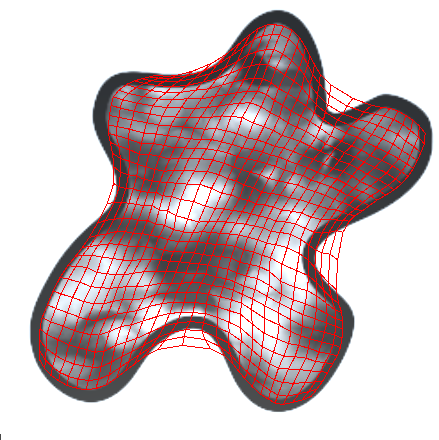
\includegraphics[width=0.475\textwidth, height=0.35\textheight, keepaspectratio]{Images/GrowingGridShape.png}
        \label{fig:growingGrid1}
    }
    \hfill
    \subfigure[Fitting WFC onto an irregular quadrilateral grid]{
        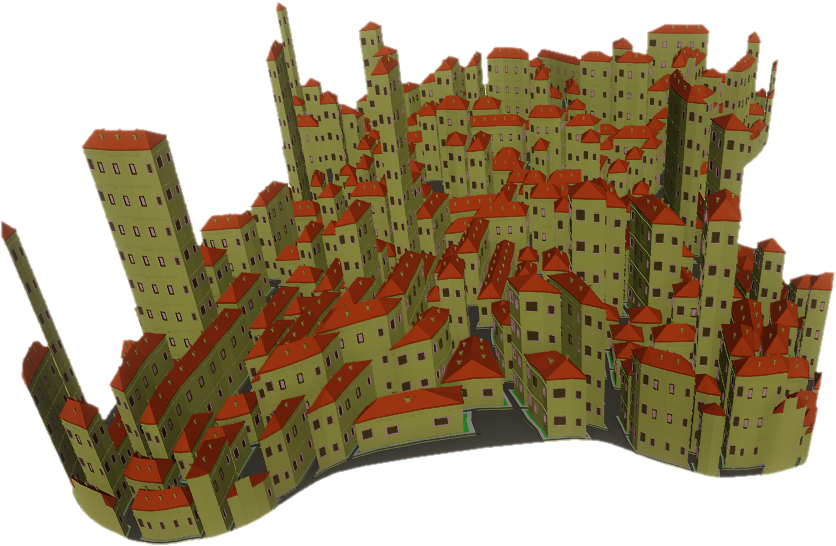
\includegraphics[width=0.475\textwidth, height=0.35\textheight, keepaspectratio]{Images/GrowingGridWFC.png}
        \label{fig:growingGrid2}
    }
    \caption{Using growing grid and WFC to generate more complex worlds \cite{WFC_Neural_Network}}
    \label{fig:growingGrid}
\end{figure}

Very simple implementations may ignore symmetry when defining tile neighbours in the simple tiled method \cite{Easy_WFC}. Instead, every neighbour for each direction of each tile is listed explicitly. While this keeps the code simple, it means that a huge amount of work is required when defining neighbours for complex tile sets, with high chance of human error. What the original WFC implementation and several others do instead is to define a symmetry type for each tile. This means that much less data about the input has to be provided, lessening the work required and chance of human error. The original WFC implementation defines five symmetry types, which it applies to a variety of 2D images. Another paper instead defines nine symmetry types as in Table \ref{fig:symmetryDictionary}, which supports a greater variety of tile sets \cite{WFC_Automatic_Rules_And_Better_Symmetries}.

\begin{table}[H]
    \centering
    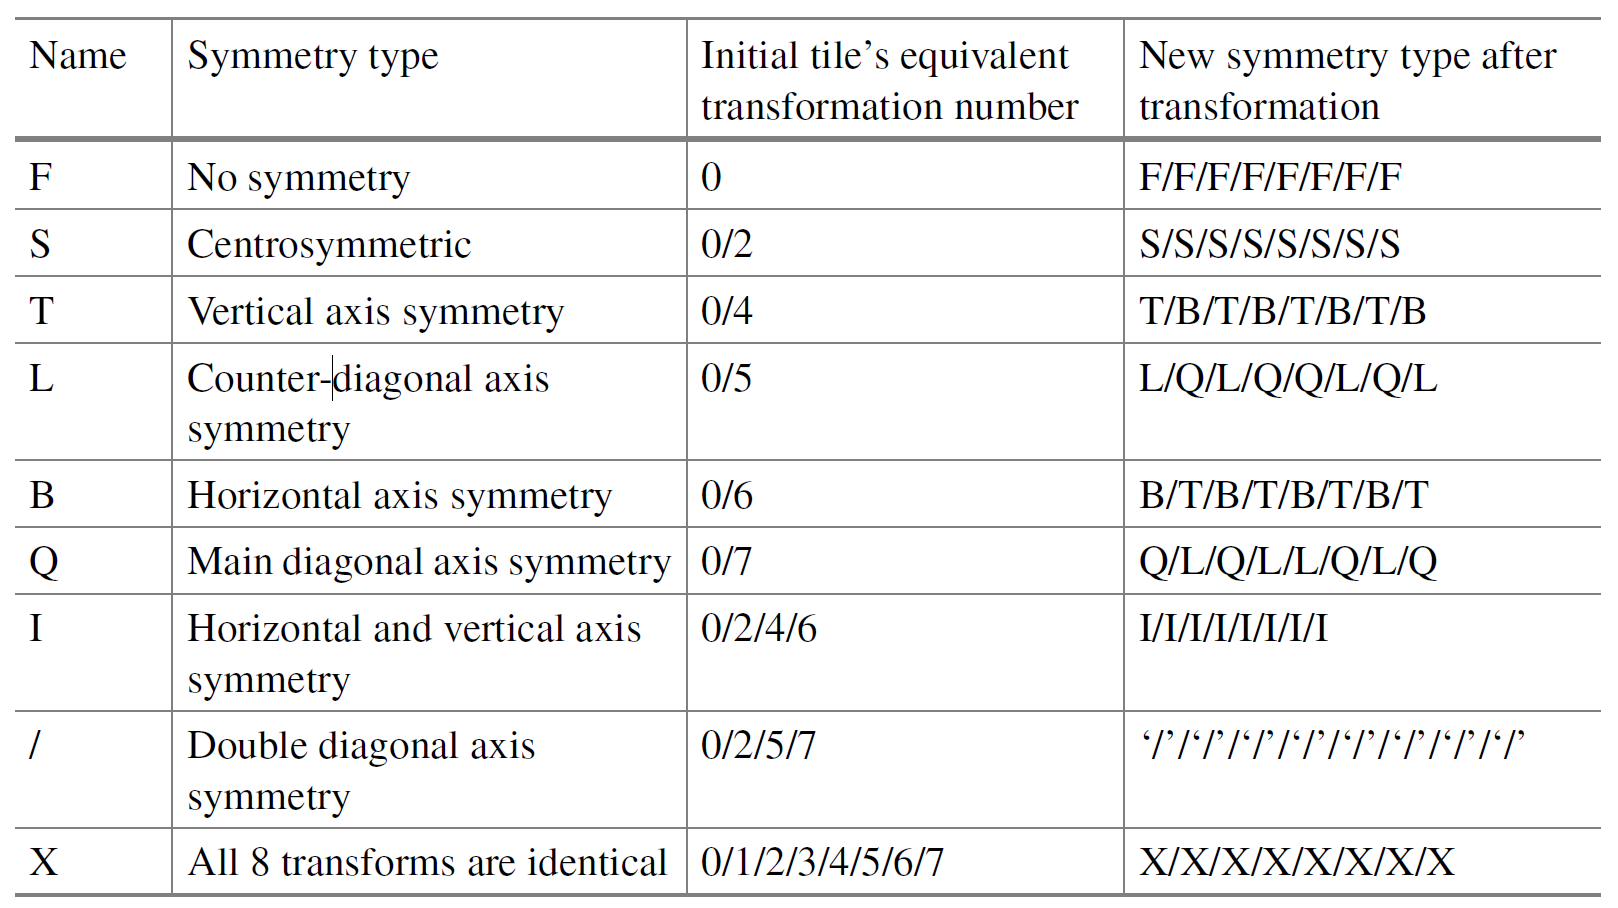
\includegraphics[width=\textwidth, height=0.3\textheight, keepaspectratio]{Images/SymmetryDictionary.png}
    \caption{A symmetry dictionary proposed by \cite{WFC_Automatic_Rules_And_Better_Symmetries}}
    \label{fig:symmetryDictionary}
\end{table}

%\subsection{Search Algorithms}
%\subsection{Generation Methods}
%There are many different generation methods used in PCG, each with specific applications. For example, a cellular automata or agent-based digger may be used to generate a dungeon or cave. Noise maps [CITE] are often used for terrain generators such as the one used in Minecraft [CITE].
